\documentclass[stu, 12pt, letterpaper, donotrepeattitle, floatsintext, natbib]{apa7}
\usepackage[utf8]{inputenc}
\usepackage{comment}
\usepackage{marvosym}
\usepackage{graphicx}

\usepackage[normalem]{ulem}
\usepackage[spanish]{babel} 
\usepackage{ragged2e}
\usepackage{xspace}
\usepackage{svg}
\usepackage{newtxtext}
\usepackage{colortbl}

%formulas
\usepackage{amsmath}

%tabla multi hoja
\usepackage{longtable}

%para bibliografia
\usepackage{url}  % Para manejar correctamente las URLs en la bibliografía
\usepackage{hyperref} % Para enlaces clicables en la versión digital

%Ajustar tablas :v
\usepackage{adjustbox}

%paquetes para las tablas
\definecolor{ChetwodeBlue}{rgb}{0.556,0.662,0.858}
\usepackage{multirow}
\usepackage{multicol}
\usepackage{color}
\usepackage{tabularray}
\UseTblrLibrary{booktabs}
\usepackage[flushleft]{threeparttable}
\usepackage{float}

%configuracion de los espacios entre titulos
\usepackage{titlesec}

%\titlespacing{\subsection}{0pt}{12pt plus 1ex minus 0.2ex}{0pt plus 0.2ex} % Espaciado solo antes de \subsection
%\titlespacing{\subsubsection}{0pt}{12pt plus 1ex minus 0.2ex}{0pt plus 0.2ex} % Espaciado solo antes de \subsubsection



% Mantener el centrado de los títulos de nivel 1
%\titleformat{\section}
%  {\normalfont\large\bfseries\centering}{\thesection}{1em}{}
%\titlespacing{\section}{0pt}{0.0ex plus 0.5ex minus .2ex}{1.5ex plus .2ex}

% Configurar espaciado de los títulos de nivel 2 (\subsection)
%\titleformat{\subsection}
%  {\normalfont\normalsize\bfseries}{\thesubsection}{1em}{}
%\titlespacing{\subsection}{0pt}{12pt plus 1ex minus 0.2ex}{0pt plus 0.2ex}

% Configurar espaciado de los títulos de nivel 3 (\subsubsection)
%\titleformat{\subsubsection}
%  {\normalfont\normalsize\bfseries}{\thesubsubsection}{1em}{}
%\titlespacing{\subsubsection}{0pt}{12pt plus 1ex minus 0.2ex}{0pt plus 0.2ex}

%Cambiar de Figura a Diagrama:
\addto\captionsspanish{\renewcommand{\figurename}{Diagrama}}

%Cambiar de Cuadro a Tablas:
\addto\captionsspanish{\renewcommand{\tablename}{Tabla}}

%para poner paginas en horizontal
\usepackage{pdflscape}


%para combinar las listas
%\usepackage{floatrow}
\usepackage{caption}

%para la ref de tablas
%\newcommand{\tableref}[1]{Tabla~\ref{#1}}

%caption de tablas*
%\addto\captionsspanish{\renewcommand{\listtablename}{Índice de tablas}}

%indice
%\addto\captionsspanish{\renewcommand{\tablename}{Tabla}}

%Espaciado doble
\usepackage{setspace}
\doublespacing

\usepackage{caption} % Para personalizar los títulos de las figuras
\usepackage{enumitem} % Para ajustar la sangría de las listas
\usepackage{changepage} % Para ajustar temporalmente el margen

\fancyhf{}
\cfoot{\thepage}

\selectlanguage{spanish}
\useunder{\uline}{\ul}{}
%\newcommand{\myparagraph}[1]{\paragraph{#1}\mbox{}\\}

% Portada
%\thispagestyle{empty}

\begin{document}

\begin{titlepage}
	\begin{center}
		
\includegraphics[width=6cm]{imagenes/senati.png}\\
		\vspace*{0.5cm}
		\textbf{SERVICIO NACIONAL DE ADIESTRAMIENTO EN TRABAJO INDUSTRIAL}\\
		\vspace*{1.5cm}
		\textbf{DIRECCIÓN ZONAL: AREQUIPA - PUNO}\\
		\textbf{Escuela/CFP: Escuela de Tecnologias de la Información}\\
		\textbf{Carrera: Ingenieria de Software con Inteligencia Artificial}\\
		\vspace*{1.8cm}
		\textbf{Proyecto de Innovación / Mejora / Creatividad\\Nivel Profesional Técnico / Técnico Operativo}\\
		\vspace*{1.7cm}
		\textbf{\LARGE Optimización y automatización de la gestión de datos e información para talleres mecánicos}\\
		\vspace*{1cm}
		\textbf{Autor:    ELIOT ROY ARIAS FLORES}\\
		\textbf{Asesor:    CESAR ROSAS ARAGÓN}\\
		\vspace*{1.5cm}
		Arequipa, Perú\\
		\textbf{2024}

	\end{center}

\end{titlepage}


\justifying
\setlength{\parindent}{1.27cm}


\pagenumbering{roman}
%Codigo para evitar la separación silabica:
\pretolerance=10000
\tolerance=100
\emergencystretch=5pt
%posdata funcion <3 

%------------dedicatoria------------
\newpage
\begin{justify}
	\begin{flushright}
		\textit{ } \\
		%\vfill
		\begin{minipage}{0.6\textwidth} % Limitar el ancho al 60% del ancho de la página

			\textit{DEDICATORIA} \\
			\textit{Dedico este trabajo a mi madre y mi familia que me apoyaron durante el proceso de aprendizaje y formación, este proyecto es el primer paso hacia el éxito profesional}
		\end{minipage}
	\end{flushright}
\end{justify}
%------------Agradecimiento------------
\newpage
\begin{justify}
	\begin{flushright}
		\textit{ } \\
		%\vfill
		\begin{minipage}{0.6\textwidth} % Limitar el ancho al 60% del ancho de la página

			\textit{AGRADECIMIENTO} \\
			\textit{Agradezco a mi familia por el apoyo durante la carrera, a mis instructores que me aconcejaron para alcanzar mis metas, a las empresas que me abrieron sus puertas para poder hacer mis practicas.}
		\end{minipage}
	\end{flushright}
\end{justify}

%---------Hoja de presentación----------
\newpage
\section*{Hoja de presentacion del aprendiz}

\begin{itemize}
    \item[] \textbf{Nombres: }Eliot Roy
    \item[] \textbf{Apellidos: }Arias Flores
    \item[] \textbf{Codigo: }001386784
    \item[] \textbf{Direccion: }Sor Ana de los Angeles Sect. 1 Mz. D Lt. 6
    \item[] \textbf{Telefono: }907487141
    \item[] \textbf{Carrera: }Ingeniera de Software con Inteligencia Artificial
    \item[] \textbf{Direccion Zonal: }Arequipa - Puno
    \item[] \textbf{CFP: }Arequipa
    \item[] \textbf{Bloque: }51PIADS601
    \item[] \textbf{Semestre: }VI
    \item[] \textbf{Año de Ingreso: }2021(20)
\end{itemize}

%-----------RESUMEN EJECUTIVO-----------
\newpage
\section*{RESUMEN EJECUTIVO DEL PROYECTO DE MEJORA}

El presente proyecto se centra en la optimización y automatización de la gestión de datos e información para talleres mecánicos, desarrollado en el marco del Servicio Nacional de Adiestramiento en Trabajo Industrial (SENATI) bajo la dirección del autor Eliot Roy Arias Flores y la asesoría de César Rosas Aragón. Este proyecto se realizó con el objetivo de mejorar la eficiencia operativa de la empresa Automotriz Pelayo S.A.C. mediante la implementación de un sistema de gestión de datos más eficiente.

En el primer capítulo, se identificaron los problemas técnicos que afectan el desempeño y la eficiencia operativa de la empresa. Utilizando herramientas como la lluvia de ideas, el diagrama de afinidades y la matriz de priorización, se evaluaron los problemas en función de su frecuencia, importancia y factibilidad. Los problemas identificados incluyeron la falta de disponibilidad de piezas, un deficiente sistema centralizado de registro, falta de personal capacitado, sobrecarga de tareas y deficiencias en la infraestructura y equipamiento del taller.

El segundo capítulo establece los objetivos del proyecto, tanto generales como específicos, con el objetivo principal de optimizar el registro y gestión de datos de la empresa. Los objetivos específicos incluyen asegurar la correcta registración de la información, eliminar duplicidades, mejorar la eficiencia en la gestión de datos, reducir errores en la facturación y fortalecer la calidad del servicio al cliente.

En el tercer capítulo se revisan los antecedentes del proyecto, analizando estudios previos y proyectos similares realizados en talleres mecánicos. Estos antecedentes proporcionan un contexto valioso y lecciones aprendidas que influyen en la formulación de estrategias y la toma de decisiones para el proyecto actual.

El cuarto capítulo justifica la necesidad del proyecto de mejora, destacando los problemas críticos actuales de la gestión de datos en Automotriz Pelayo S.A.C. La implementación de este proyecto es crucial para mejorar la precisión y eficiencia operativa, aumentar la satisfacción del cliente, fortalecer la competitividad de la empresa y optimizar el uso de recursos.

El quinto capítulo presenta el marco teórico y conceptual del proyecto, abordando temas clave como SQL y bases de datos, el desarrollo backend y frontend, y herramientas como Spring Boot y Angular. También se explican conceptos fundamentales relacionados con la eficiencia operativa y la satisfacción del cliente, que son esenciales para la implementación exitosa del proyecto.

El sexto capítulo detalla el plan de acción de la mejora propuesta, incluyendo las tareas, recursos necesarios, cronograma de ejecución y posibles limitaciones que podrían surgir. La planificación detallada y la asignación de responsabilidades claras son esenciales para asegurar una implementación eficiente y efectiva del proyecto.

Finalmente, el séptimo capítulo evalúa los costos de implementación, incluyendo materiales, recursos humanos, equipos y otros gastos relevantes. Este análisis proporciona una visión completa de los recursos financieros necesarios para llevar a cabo la mejora con éxito, asegurando la viabilidad y sostenibilidad del proyecto.

En conclusión, el proyecto de mejora ha logrado una optimización efectiva en el registro y gestión de datos en Automotriz Pelayo S.A.C., eliminando duplicidades, mejorando la precisión y eficiencia en la recuperación de información, y fortaleciendo la calidad del servicio al cliente.


%\subsection{Introducción}
%
%El presente proyecto se centra en la optimización y automatización de la gestión de datos e información para talleres mecánicos. Este trabajo se ha realizado en el marco del Servicio Nacional de Adiestramiento en Trabajo Industrial (SENATI), dentro de la Escuela de Tecnologías de la Información, y ha sido desarrollado por Eliot Roy Arias Flores bajo la asesoría de César Rosas Aragón.
%
%
%\subsection*{Objetivos del Proyecto}
%El objetivo general del proyecto es optimizar el registro y gestión de datos de la empresa para mejorar la eficiencia operativa. Los objetivos específicos incluyen:
%
%\begin{enumerate}
%    \item Asegurar la correcta registración de la información de clientes y servicios.
%    \item Eliminar la duplicidad de registros y mejorar la precisión de la información.
%    \item Implementar prácticas para una búsqueda y recuperación más eficiente de la información.
%    \item Agilizar y aumentar la precisión en el proceso de facturación.
%    \item Fortalecer la calidad del servicio al cliente, asegurando que los datos sean accesibles y actualizados.
%\end{enumerate}
%
%\subsection*{Metodología}
%La metodología del proyecto se basa en un análisis detallado de los problemas técnicos actuales, seguido de la identificación de objetivos de mejora, la implementación de soluciones tecnológicas, y la evaluación de los resultados obtenidos. Se han utilizado herramientas como bases de datos SQL, frameworks de desarrollo backend y frontend (Spring Boot y Angular), y técnicas de mapeo objeto-relacional y APIs REST.
%
%
%\subsection*{Resultados Esperados}
%Se espera que la implementación del proyecto resulte en un ahorro significativo de tiempo y recursos, mejorando la eficiencia en la gestión de datos y la calidad del servicio al cliente. Los beneficios económicos se derivarán principalmente del ahorro en mano de obra y la reducción de errores en la facturación.
%
%
%\subsection*{Conclusiones}
%El proyecto ha concluido con éxito, cumpliendo con los objetivos propuestos. Se ha logrado una optimización efectiva en el registro y gestión de datos, eliminando duplicidades y mejorando la precisión y eficiencia en la recuperación de información. Además, se ha fortalecido la calidad del servicio al cliente, proporcionando un acceso más rápido y preciso a la información relevante.
%----------INDICE------------
\newpage
%\pagenumbering{roman}
% Contenido
\renewcommand{\contentsname}{Índice de contenido}
\tableofcontents
\setcounter{tocdepth}{1}



% Fíguras a diagramas
\renewcommand{\listfigurename}{Índice de diagramas}
\newpage
\listoffigures
%\listoffigures

% Tablas 
\renewcommand{\listtablename}{Índice de tablas}
\newpage
\listoftables

% Cuerpo
%\pagenumbering{arabic}


\newpage
\pagenumbering{arabic}




%-----------CAPITULO 1-----------
\newpage
\section{Capitulo I}
\section*{Generalidades de la empresa}
En este primer capitulo, se proporciona un análisis detallado de las generalidades de la empresa. Se examinaran aspectos clave como su razón social, RUC, y gerencia, así como su misión, visión y valores fundamentales que guían su operación. Además se describirán los servicios ofrecidos por la empresa, el mercado en el que opera y los clientes principales a los que se dirige.
\subsection{1.1 Razón social}
En esta sección se proporciona la información general de la empresa, como la gerencia; razón social; dirección; ruc; principal actividad económica; logo y ubicación.
\begin{itemize}
    \item[] \textbf{GERENTE GENERAL: }CARCAUSTO HUACHANI GUSTAVO ADOLFO
    \item[] \textbf{RAZÓN SOCIAL: } AUTOMOTRIZ PELAYO S.A.C.
    \item[] \textbf{DIRECCION: } MERCURIO MZA. K LOTE. 3 CAMPO MARTE ZONA A AREQUIPA - AREQUIPA - PAUCARPATA
    \item[] \textbf{RUC:} 20605004726    
    \item[] \textbf{ACTIVIDAD ECONÓMICA: }MANTENIMIENTO Y REPARACIÓN DE VEHÍCULOS AUTOMOTORES
\end{itemize}
\begin{figure}[h]
    \centering
        \captionsetup{singlelinecheck=false}
    \caption*{Logo de la Empresa}
    
\includegraphics[width=5cm]{imagenes/logo.png}
    \label{fig:logo}
\end{figure}
\newpage

\subsection{1.2 Misión, Visión, Objetivos, Valores de la empresa}
Esta sección proporciona una comprensión de la dirección y los principios fundamentales de la empresa, a través de la misión se destaca su compromiso con el mejor desenvolvimiento en su rubro, mientras la visión enfatiza su aspiración de liderazgo en el sector. Los objetivos establecen las metas especifícas para su mejora en la atención al cliente, y los valores fundamentales que guían las acciones de la empresa.
\subsubsection*{1.2.1 Misión}
Nos dedicamos a proporcionar servicios de mantenimiento mecánico de primera calidad para una amplia variedad de vehículos y maquinaria. Nuestro compromiso es superar constantemente las expectativas de nuestros clientes, ofreciendo soluciones integrales, confiables y eficientes. Además, nos comprometemos a promover un ambiente de trabajo seguro, colaborativo y profesional para nuestro equipo, fomentando el crecimiento personal y profesional de nuestros empleados.
\subsubsection*{1.2.2 Visión}
Buscamos ser reconocidos como líderes en el sector automotriz y de mantenimiento mecánico, Buscamos destacarnos no solo por nuestra excelencia en el servicio al cliente, sino también por nuestro firme compromiso con la innovación y la mejora continua. Aspiramos a inspirar confianza y seguridad en cada interacción con nuestros clientes.


\subsubsection*{1.2.3 Objetivos de la Empresa}
%Explicar
Los objetivos de la empresa son metas específicas que guían la dirección estratégica y orientan sus acciones hacia los resultados deseados. Representan los logros cuantitativos y cualitativos que la empresa busca alcanzar en un período determinado, proporcionando un marco para la toma de decisiones y la asignación de recursos. Estos objetivos son fundamentales para establecer una visión clara del camino hacia el éxito y para medir el progreso de la empresa en su conjunto.


\paragraph{Objetivo Principal. }Incrementar la satisfacción y el numero de clientes, así como la rentabilidad de la empresa.
\paragraph{Objetivos Secundarios. }Los siguientes objetivos secundarios desglosan el objetivo principal en áreas clave como la expansión de la clientela, la mejora operativa y la calidad del servicio, asegurando que cada aspecto contribuya al éxito y satisfacción del cliente.
\begin{itemize}
    \item Ampliar la cartera de clientes aumentando el número de clientes durante el próximo trimestre.
    \item Mejorar la eficiencia operativa reduciendo tiempos de espera mediante la optimización de los procesos operativos.
    \item Mejorar la calidad de servicios ofrecidos.
\end{itemize}

\subsubsection*{1.2.4 Valores de la Empresa}
%Explicar 
Los valores de una empresa son principios éticos fundamentales que establecen la cultura de la organización y permiten crear pautas de comportamiento coherentes. En el caso de AUTOMOTRIZ PELAYO S.A.C., los valores centrales que guían todas las operaciones y decisiones son:
\begin{enumerate}
    \item Calidad: Compromiso con la excelencia en la ejecución de cada servicio, asegurando la máxima calidad en cada tarea realizada.
    \item Integridad: Actuar con honestidad, transparencia y ética en todas las interacciones con clientes, empleados y socios comerciales.
    \item Compromiso con el cliente: Priorizar las necesidades y la satisfacción del cliente, ofreciendo soluciones personalizadas y un servicio excepcional.
    \item Profesionalismo: Actuar con responsabilidad y diligencia en cada tarea.
    \item Seguridad: Priorizar la seguridad de los empleados y clientes en todas las operaciones y actividades de la empresa.
\end{enumerate}
\subsection{1.3 Servicios, mercado, clientes}
La siguiente sección abordará los servicios ofrecidos por AUTOMOTRIZ PELAYO S.A.C., así como el mercado al que se dirige y sus principales clientes. En cuanto a los servicios, se proporcionará un detalle de las distintas categorías de mantenimiento y reparación mecánica ofrecidos. Se explicará cómo estos servicios contribuyen a satisfacer las necesidades de los clientes. Además, se analizará el mercado local en el que opera la empresa. Se describirá el contexto del mercado de servicios de mantenimiento mecánico y reparación de vehículos y maquinaria. Finalmente, se identificarán los principales clientes de la empresa, clasificándolos en clientes privados e industriales.

\subsubsection*{1.3.1 Servicios}
AUTOMOTRIZ PELAYO S.A.C. ofrece una gama completa de servicios de mantenimiento y reparación mecánica, diseñados para satisfacer las diversas necesidades de sus clientes. La empresa se especializa en el cuidado y mantenimiento de vehículos y maquinaria, brindando soluciones integrales que aseguran un rendimiento óptimo y prolongan la vida útil de los equipos. A continuación, se detalla la oferta de servicios, dividida en dos categorías principales: mantenimiento mecánico y reparación.

\paragraph{Servicios de Mantenimiento Mecánico. }Estos servicios están diseñados para mantener los vehículos y maquinaria en condiciones óptimas de funcionamiento y prevenir posibles fallos. Incluyen una serie de acciones preventivas que ayudan a identificar y corregir problemas antes de que se conviertan en averías mayores, asegurando así una mayor eficiencia y seguridad operativa: 
\begin{itemize}
    \item Mantenimiento preventivo para vehículos y maquinaria.
    \item Cambios de aceite y filtros.
    \item Lubricación de piezas y componentes.
    \item Servicios de diagnóstico y revisión periódica.
\end{itemize}
\paragraph{Servicios de Reparación. }AUTOMOTRIZ PELAYO S.A.C. ofrece una serie de servicios de reparación para corregir y solucionar problemas mecánicos y eléctricos en vehículos y maquinaria. Estos servicios están destinados a restablecer el funcionamiento normal y seguro de los equipos, incluyendo reparaciones específicas y la sustitución de componentes defectuosos, así como la restauración de la estructura y la estética de los vehículos.
\begin{itemize}
    \item Reparación de sistemas mecánicos y eléctricos de vehículos y maquinaria.
    \item Sustitución de piezas y componentes defectuosos.
    \item Solución de problemas específicos o averías.
    \item Reparación de daños estructurales.
    \item Servicios de pintura y restauración
\end{itemize}

\subsubsection*{1.3.2 Mercado}
%La empresa AUTOMOTRIZ PELAYO S.A.C. opera en el mercado local de servicios de mantenimiento mecánico y reparación de vehículos y maquinaria en la región de Arequipa.
AUTOMOTRIZ PELAYO S.A.C. opera en el mercado local de servicios de mantenimiento mecánico y reparación de vehículos y maquinaria en la región de Arequipa. Este mercado está compuesto principalmente por consumidores y empresas de la región que requieren servicios especializados para el mantenimiento y la reparación de sus vehículos. La empresa se enfoca en satisfacer la demanda, ofreciendo soluciones adaptadas a las necesidades específicas de los clientes en la zona, lo que le permite competir eficazmente en un entorno donde la proximidad y la calidad del servicio son cruciales para el éxito.


\subsubsection*{1.3.3 Clientes Principales}
Identificar y comprender a los principales clientes de AUTOMOTRIZ PELAYO S.A.C. es clave para desarrollar estrategias que respondan efectivamente a sus necesidades. Los clientes de la empresa se dividen en dos categorías principales: clientes privados e industriales, cada uno con características y requisitos específicos que la empresa busca satisfacer mediante sus servicios especializados:

\paragraph{Clientes Privados. }Los clientes privados de AUTOMOTRIZ PELAYO S.A.C. son individuos que poseen vehículos particulares y requieren servicios de mantenimiento y reparación para mantener sus automóviles en óptimas condiciones. Estos clientes buscan soluciones confiables y de calidad para garantizar la seguridad y el buen funcionamiento de sus vehículos. La empresa se compromete a ofrecer un servicio personalizado y eficiente que satisfaga las expectativas de cada propietario de vehículo.
 
\begin{itemize}
    \item Propietarios de vehículos particulares: Estos clientes son propietarios individuales de vehículos que requieren servicios de mantenimiento y reparación para sus automóviles personales.
\end{itemize}

\paragraph{Clientes Industriales. }Los clientes industriales de AUTOMOTRIZ PELAYO S.A.C. incluyen empresas que poseen flotas de vehículos o maquinaria pesada y requieren servicios de mantenimiento y reparación para garantizar la continuidad y eficiencia de sus operaciones. Estos clientes valoran la capacidad de la empresa para manejar servicios complejos y su habilidad para ofrecer soluciones a medida que aseguren la operatividad y longevidad de sus equipos.

\begin{itemize}
    \item Empresas de transporte: Incluye empresas dedicadas al transporte de mercancías o pasajeros que requieren servicios de mantenimiento y reparación para su flota de vehículos comerciales. 
    \item Empresas industriales con maquinaria: Comprende empresas que operan maquinaria industrial y requieren servicios de mantenimiento mecánico para garantizar el funcionamiento óptimo de sus equipos.
    \item Talleres mecánicos: Otros talleres mecánicos pueden subcontratar servicios especializados a AUTOMOTRIZ PELAYO S.A.C. cuando enfrentan tareas que están fuera de su experiencia o capacidad. 
\end{itemize}

%Estructura 
\subsection{1.4 Estructura de la Organización}
La estructura de la organización define técnicamente las relaciones que deben existir entre las funciones, niveles y actividades de las personas con el fin de lograr máxima eficiencia en la realización de planes y objetivos.
En la parte superior de este organigrama se encuentra el gerente general, quien está a cargo de la gestión global de la empresa. Bajo el gerente general, se encuentra el gerente de sucursal, este asu vez lidera la sucursal de la empresa. A su vez, el gerente de sucursal supervisa a un técnico, quien es responsable de llevar a cabo las actividades técnicas y operativas en su respectiva sucursal. Esta organizacion se repite en cada una de las 3 sucursales que tiene la empresa.

%\begin{figure}[H]
%    \centering
%    \caption{Organigrama de la empresa}
%    \label{organigrama}
%    \includesvg[width=15cm]{imagenes/Organigrama.svg}
%\end{figure}

\begin{figure}[H]
    \centering
    \caption{Organigrama de la empresa}
    \label{organigrama}
    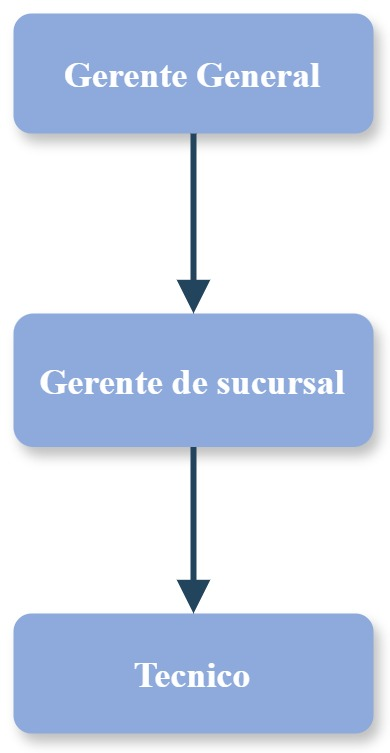
\includegraphics[width=6cm, height=10cm]{imagenes/cap1/Organigrama123.jpg}
\end{figure}

\subsection{1.5 Otra información relevante de la empresa donde se desarrolla el proyecto.}
La empresa Automotriz PELAYO S.A.C. se estableció en el año 2019 fundada por el Sr. Gustavo Adolfo Carcausto Huachani, con una amplia experiencia trabajando en varios talleres, hasta que decidió emprender su propio negocio.
Actualmente, la empresa ha demostrado un compromiso constante con la excelencia en el servicio al cliente y la calidad en sus operaciones. Además se enorgullece de mantener relaciones sólidas con proveedores de repuestos y materiales de alta calidad, garantizando así la fiabilidad y durabilidad de sus servicios.
El Gerente General sostiene que como empresa automotriz, su objetivo es satisfacer los requerimientos y expectativas de los clientes, gestionando eficientemente los recursos y procesos. Además, buscan prevenir incidentes, enfermedades ocupacionales, impactos ambientales y conflictos sociales, promoviendo una cultura de seguridad y mantenibilidad. También se comprometen a cumplir con la legislación nacional y normas vigentes relacionadas con la calidad, seguridad, salud, ambiental y social aplicables a sus operaciones.

%-----------CAPITULO 2-----------
\newpage
\section{Capitulo II}
\section*{Plan del proyecto de mejora}
%Introduccion del cap 2
En este capítulo, se aborda el análisis y la planificación de las acciones para resolver los problemas identificados en Automotriz PELAYO S.A.C. Se inicia con la identificación detallada de los problemas técnicos utilizando diversas herramientas como la lluvia de ideas y la matriz de priorización. Luego, se establecen los objetivos del proyecto, se revisan antecedentes relevantes y se justifica la necesidad de llevar a cabo el proyecto de mejora. Este capítulo sienta las bases para el desarrollo de acciones concretas que mejorarán la eficiencia operativa y la satisfacción del cliente en la empresa.

\subsection{2.1 Identificación del problema técnico en la empresa}
%Introduccion de la subsection 2.1
En este punto, se llevará a cabo un análisis detallado de los problemas técnicos que afectan el desempeño y la eficiencia operativa de la empresa. Se utilizarán diversas herramientas y técnicas, como la lluvia de ideas, el diagrama de afinidades y la matriz de priorización, para identificar y priorizar estos problemas de manera sistemática.\\
Se examinarán áreas clave de la empresa, como la disponibilidad de recursos humanos, la infraestructura y el equipamiento, así como la gestión de la información. Cada problema técnico identificado será evaluado en función de su frecuencia, importancia y factibilidad, permitiendo una comprensión más profunda de su impacto y urgencia.

\subsubsection*{2.1.1 Trabajo en Equipo}
Para abordar el problema técnico identificado en la empresa, se aplicará la técnica de trabajo en equipo. Esta estrategia implica la participación activa de todos los miembros del personal,
el objetivo es aprovechar la experiencia y el conocimiento de cada uno de ellos para comprender mejor el problema desde diferentes perspectivas.
\subsubsection*{2.1.2 Lluvia de Ideas}
Se empleo la técnica de lluvia de ideas para poder identificar el problema técnico de la empresa. Esta metodología, tiene como objetivo que los participantes aporten sobre los problemas que tienen al realizar su trabajo diario, esta fue la lista de problemas que cada participante indico que tiene en la realización de su trabajo.
\begin{enumerate}
    \item Falta de disponibilidad de piezas y componentes:
    \begin{itemize}
        \item Problema: No se dispone de las piezas y componentes necesarios para realizar las reparaciones de manera oportuna.
        \item Impacto: Aumento en el tiempo de espera para los clientes, disminución de la satisfacción del cliente, y retrasos en la entrega de servicios.
    \end{itemize}    

    \item Deficiente sistema centralizado de registro:
    \begin{itemize}
        \item Problema: La información de los clientes y de los servicios ofrecidos no está bien centralizada, lo que dificulta su acceso y gestión.
        \item Impacto: Ineficiencia en la búsqueda de información, duplicidad de registros y dificultades para ofrecer un servicio al cliente coherente y eficiente.
    \end{itemize}
    
    \item Falta de personal capacitado para tareas específicas:
    \begin{itemize}
        \item Problema: El taller carece de personal con la formación y habilidades necesarias para realizar tareas especializadas.
        \item Impacto: Menor calidad en los servicios ofrecidos, aumento en los errores y trabajos repetidos, y dependencia de personal externo o de otros talleres.
    \end{itemize}
    
    \item Exceso de tareas en cola para el personal:
    \begin{itemize}
        \item Problema: El personal del taller tiene una gran cantidad de tareas acumuladas, lo que dificulta la gestión eficiente del tiempo y los recursos.
        \item Impacto: Aumento en los tiempos de espera para los servicios, incremento en la carga de trabajo del personal y potencial disminución de la calidad del trabajo debido a la sobrecarga.
    \end{itemize}

    \item Deficiencia en la gestión de tiempo de los operarios:
    \begin{itemize}
        \item Problema: La falta de una adecuada planificación y organización del tiempo de los operarios lleva a una gestión ineficiente de las tareas.
        \item Impacto: Menor productividad, retrasos en la finalización de trabajos y posible pérdida de clientes debido a la falta de puntualidad en la entrega de servicios.
    \end{itemize}

    \item Deficiencias en la infraestructura y equipamiento del taller:
    \begin{itemize}
        \item Problema: La infraestructura y el equipamiento del taller son inadecuados o insuficientes para satisfacer la demanda de servicios.
        \item Impacto: Aumento en los tiempos de reparación, limitaciones en la capacidad de servicio y posibles inconvenientes en la calidad del trabajo realizado.
    \end{itemize}

    \item Retrasos en la entrega de servicios debido a carga de trabajo excesiva:
    \begin{itemize}
        \item Problema: La alta demanda de servicios sobrecarga la capacidad del taller, resultando en retrasos.
        \item Impacto: Insatisfacción del cliente, pérdida de clientes potenciales y estrés laboral para los empleados.
    \end{itemize}

    \item Dificultades para gestionar la demanda en períodos de alta actividad:
    \begin{itemize}
        \item Problema: El taller enfrenta dificultades para manejar la alta demanda de servicios durante las temporadas pico, como vacaciones o épocas de mal tiempo.
        \item Impacto: Incremento en los tiempos de espera, baja calidad en el servicio debido a la presión y potencial pérdida de clientes.
    \end{itemize}
    
    \item Retrasos en la facturación:
    \begin{itemize}
        \item Problema: El proceso manual de facturación puede ser lento y propenso a errores.
        \item Impacto: Demoras en la emisión de facturas, insatisfacción de los clientes y posibles problemas de flujo de caja debido a la tardanza en la recepción de pagos.
    \end{itemize}    
    
    \item Falta de mantenimiento regular de las herramientas y equipos:
    \begin{itemize}
        \item Problema: Las herramientas y equipos del taller no reciben mantenimiento adecuado y regular, lo que puede llevar a fallos y a la necesidad de reparaciones frecuentes.
        \item Impacto: Retrasos en la realización de servicios, incremento en los costos operativos y posible disminución en la calidad del trabajo debido a herramientas defectuosas.    
    \end{itemize}    
\end{enumerate}

\subsubsection*{2.1.3 Diagrama de Afinidades}
En este punto se diseñará el diagrama de afinidades en base a la lluvia de ideas generada en el punto anterior. De esta forma, se agruparán los elementos relacionados en categorías clave, facilitando la identificación de soluciones específicas para cada problema. Las categorias elegidas son estas:%El siguiente diagrama divide las ideas, en tres conceptos clave, Registro y Gestión de Datos, gestión de Recursos Humanos e Infraestructura y Equipamiento. De esta forma se facilitará la identificación de soluciones efectivas para cada categoría de problemas.
%tabla 1 para referenciar
\begin{itemize}
    \item Registro y Gestión de Datos: Incluye problemas relacionados con la falta de disponibilidad de piezas y componentes necesarios para las reparaciones, retrasos en la facturación debido a procesos manuales y la falta de un sistema centralizado para el registro de información.
    \item Gestión de Recursos Humanos: Abarca la falta de personal capacitado, la sobrecarga de tareas para el personal y la deficiencia en la gestión del tiempo de los operarios, lo que afecta la calidad del servicio y la eficiencia del taller.
    \item Infraestructura y Equipamiento: Se refiere a las deficiencias en la infraestructura del taller y en el equipamiento, la dificultad para gestionar la alta demanda de servicios y la falta de mantenimiento regular de herramientas y equipos, lo que puede aumentar los costos operativos y provocar retrasos en la entrega de servicios.
\end{itemize}


\definecolor{ChetwodeBlue}{rgb}{0.556,0.662,0.858}
\begin{table}[H]
\caption[Diagrama de afinidades]{Diagrama de afinidades}
\label{tab:afinidides}
\centering
\begin{threeparttable}
\begin{tblr}{
  row{1} = {ChetwodeBlue},
  cell{2}{1} = {r=3}{},
  cell{5}{1} = {r=3}{},
  cell{8}{1} = {r=4}{},
  vlines,
  hline{1-2,5,8,12} = {-}{},
  hline{3-4,6-7,9-11} = {2}{},
  column{1} = {4cm},
  column{2} = {11cm}
}
\textbf{Categoría} & \textbf{Problema}\\
Registro y Gestión de Datos & Dificultades para gestionar la demanda en períodos de alta actividad.\\
 & Retrasos en la facturación debido al proceso
  manual y propenso a errores.\\
 & Deficiente sistema centralizado de registro.\\
Gestión de Recursos Humanos & Falta
  de personal capacitado para tareas específicas.\\
 & Exceso de tareas en cola para el personal.\\
 & Deficiencia
  en la gestión de tiempo de los operarios.\\
Infraestructura y Equipamiento & Deficiencias en
  la infraestructura y equipamiento del taller.\\
 & Retrasos en la entrega de servicios debido a carga de trabajo excesiva\\
 & Falta de disponibilidad de piezas y componentes necesarios para realizar las reparaciones de manera oportuna.\\
 & Retrasos en la entrega de servicios.
\end{tblr}
\begin{tablenotes}
    %\vspace{0.1cm}
    %\footnotesize
    %\item[1] Nota al pie 1: Esta es una descripción detallada de la nota al pie 1.
    %\item[2] Nota al pie 2: Esta es una descripción detallada de la nota al pie 2.
\end{tablenotes}
\end{threeparttable}
\end{table}

\subsubsection*{2.1.4 Matriz de priorización}
%La matriz de priorización es una herramienta que mediante filas y columnas ayuda a comparar y seleccionar las prioridades entre diversas opciones o posibles soluciones, lo que hace que tomar una decisión sea mucho más sencillo. De esta forma, el diagrama de priorización permite evaluar diferentes alternativas u opciones puntuándolas respecto a criterios de interés para un problema.\citep{matrizPriorizacion}\\
Después de identificar y agrupar los problemas técnicos mediante la lluvia de ideas y el diagrama de afinidades, Ahora se debe priorizar los problemas identificados para saber que resolver primero. La matriz de priorización es utilizada para determinar qué problemas deben ser abordados primero, basándonos en su impacto y viabilidad.\\

En esta sección, se presenta la aplicación de la matriz de priorización, utilizando datos de una encuesta realizada a seis empleados directamente involucrados. Este enfoque garantiza que las decisiones de mejora se tomen de manera informada y estratégica, optimizando así el uso de los recursos disponibles.

%tabla 2 para referenciar
\begin{table}[H]
\centering
\caption[Matriz de Priorización]{Matriz de Priorización}
\begin{adjustbox}{margin=6.4cm 0cm 0cm 0cm,center} % Ajuste de márgenes: izquierda, abajo, derecha, arriba
\begin{threeparttable}
\begin{tblr}{
  row{1} = {ChetwodeBlue},
  hlines,
  vlines,
}
Ideas Base & Frec\textsuperscript{1} & Imp\textsuperscript{2} & Fact\textsuperscript{3} & Total\\
Registro y Gestión de Datos & 30 & 26 & 30 & 86\\
Gestión de Recursos Humanos & 18 & 26 & 20 & 62\\
Infraestructura y Equipamiento & 20 & 30 & 20 & 64
\end{tblr}
\begin{tablenotes}
    \vspace{0.2cm}
    \footnotesize
    \item[1]Frecuencia
    \item[2]Impacto.
    \item[3]Factibilidad.
\end{tablenotes}
\end{threeparttable}
\end{adjustbox}
\end{table}

Basándonos en la matriz de prioridades, se puede concluir que el problema principal identificado en la empresa Automotriz Pelayo S.A.C. se relaciona con el \textbf{Registro y Gestión de Datos}. Actualmente, la información de los clientes y los servicios ofrecidos no está eficientemente organizada ni centralizada, lo que dificulta su acceso y gestión por parte del personal. La ineficiencie del sistema actual también afecta a la la facturación y aumenta de los tiempos de espera para los clientes. Otras concecuencias son:
%Esté área obtuvo el puntáje más alto en los criterios de frecuencia (28), importancia(24), factibilidad, sumando un total de 82, es decir, que los problemas relacionados con la ineficiencia del sistema actual de registro y gestión de datos, es el problema más urgente a resolver.
\begin{itemize}
    \item Ineficiencia en la búsqueda de información, lo que resulta en tiempos de respuesta prolongados y retrasos en la entrega de servicios.
    \item Duplicidad de registros y posibles errores en la documentación.
    \item Dificultades para ofrecer un servicio al cliente coherente y eficiente debido a la falta de acceso rápido a la información relevante.
\end{itemize}

%Especificar el problema, 


\subsection{2.2 Objetivos del Proyecto de Mejora}
Para abordar los problemas presentes en la empresa, es necesario establecer objetivos generales y específicos que guíen las acciones del proyecto de mejora. En esta sección se definirán estos objetivos que se orientaran a resolver el problema principal.

\subsubsection*{Objetivo General:}
Optimizar el registro y gestión de datos de la empresa.
\subsubsection*{Objetivos Específicos: } 
    \begin{itemize}
        \item Optimizar el registro de datos:
        \begin{itemize}
            \item Asegurar que la información de los clientes y servicios esté correctamente registrada para facilitar su acceso y gestión.
            \item Eliminar la duplicidad de registros y mejorar la precisión de la información almacenada.
        \end{itemize}        
        
        \item Mejorar la eficiencia en la gestión de datos:
        \begin{itemize}
            \item Implementar prácticas que permitan una búsqueda y recuperación más eficiente de la información.
            \item Garantizar la coherencia y exactitud de los datos utilizados en todos los procesos operativos.
        \end{itemize}        

        \item Reducir los errores en la facturación:
        \begin{itemize}
            \item Agilizar el proceso de facturación para minimizar los retrasos en la emisión de facturas.
            \item Aumentar la precisión en la facturación para evitar errores y disputas con los clientes.
        \end{itemize}        
        
        \item Fortalecer la calidad del servicio al cliente:
        \begin{itemize}
            \item Asegurar que los datos de los clientes sean fácilmente accesibles para mejorar la respuesta a consultas y solicitudes.
            \item Mantener actualizada la información del cliente para proporcionar un servicio más personalizado y eficiente.
        \end{itemize}        
    \end{itemize}
    
\subsection{2.3 Antecedentes del Proyecto de Mejora (Investigaciones realizadas): }
Para el desarrollo efectivo de un proyecto de mejora, es esencial analizar y comprender los antecedentes que han influido en el campo de estudio. Estos antecedentes incluyen  trabajos previos, investigaciones y estudios que están directamente relacionados con los objetivos y el alcance del proyecto en curso.
%En el proceso de desarrollo de un proyecto de mejora, es crucial comprender y analizar los antecedentes que han influido en el ámbito de estudio. Estos antecedentes abarcan una amplia gama de trabajos previos, investigaciones y estudios que guardan relación con los objetivos y el alcance del proyecto actual. Constituyen una base de conocimientos y experiencias que proporcionan un contexto valioso para la formulación de estrategias y la toma de decisiones.
En esta sección, se llevará a cabo un análisis de los antecedentes relevantes, reconociendo la contribución de cada trabajo citado. 

\subsubsection*{Antecedente 1:}
%empezar con la cita.
En un estudio realizado en un taller automotriz ubicado en Lizardo García 2614, entre Colombia y Venezuela, se identificaron varios problemas relacionados con la gestión de sus procesos, los cuales se manejaban utilizando hojas de Excel . Este enfoque causaba una serie de conflictos, tales como pérdidas económicas debido a la falta de un registro automatizado de los ingresos y salidas de materiales, y pérdida de tiempo para los clientes que solicitaban informes de sus últimas visitas . Además, en caso de presentarse algún inconveniente respecto al servicio prestado, no era posible identificar de inmediato a los responsables, lo que generaba descontento tanto en los clientes como en el propietario del negocio con respecto a sus empleados.\\
Para abordar estos problemas, se propuso la tesis titulada “Análisis y Desarrollo de un Sistema de Control y Ficha Técnica de Taller Automotriz”, que presentó una solución basada en una aplicación web. Esta aplicación se diseñó para mejorar la metodología de control y seguimiento de los procesos del taller, apoyando aspectos clave como la facturación, la petición, la venta y la adquisición de productos necesarios para brindar un servicio eficiente a los clientes . La investigación se fundamentó en una metodología descriptiva, con técnicas de campo aplicadas a una población de 57 empleados del taller, de los cuales se tomó una muestra de 50 . La implementación del sistema se llevó a cabo utilizando Visual Studio 2010, el lenguaje de programación C\#, y la base de datos SQL Server 2008 R2, complementados con CSS y HTML para mejorar la visualización .
La mejora en la calidad del servicio derivada de este sistema benefició principalmente a los clientes y, por ende, a la empresa en su conjunto .

\begin{flushright}
{Fuente: \citep{antecedente1Tesis}}
\end{flushright}
%Para el estudio realizado se trabaja con un taller automotriz ubicada en Lizardo García 2614 entre Colombia y Venezuela se encargan de brindar servicios automotriz a la ciudadanía en general estos manejan sus procesos empleando hojas de Excel que les ocasiona ciertos conflictos como:
%Pérdida económicas puesto que no se posee un registro automatizado de los ingresos y salidas de materiales. Pérdida de tiempo por parte del cliente, en caso de que este solicite un informe de sus últimas visitas. En caso de presentarse algún inconveniente con respecto al servicio prestado, no se podrá conocer de forma inmediata los responsables generando con esto un descontento por parte del cliente y del dueño del negocio para con sus empleados. Observando cada uno de estos puntos y luego de un análisis e interpretación de los datos de investigación se presenta la propuesta de tesis Análisis y Desarrollo de un Sistema de Control y Ficha Técnica de Taller Automotriz, la aplicación web establece una metodología para el control y seguimiento de los procesos que se llevan a cabo dentro de un local de servicios para apoyar el tema de facturación, petición, venta y adquisición de productos involucrados en brindar atención de manera eficiente a los clientes. El estudio se basa en una metodología de investigación descriptiva, con técnicas de campo, trabajando sobre la población de los empleados del taller automotriz que son alrededor de 57 empleados, y como muestra 50 de estos. Al mejorar la calidad de servicio que brinda el establecimiento los principales beneficiarios serán los clientes y con esto la empresa en general.
%Para la realización del sistema se emplea Visual Studio 2010, lenguaje de programación C\#, y como base de datos SQL Server 2008 R2, y para mejorar la visualización del mismo se trabaja con el apoyo de CSS y HTML.\noindent \citep{antecedente1}

\subsubsection*{Antecedente 2:}
%incluir la cita antes.
%El proyecto de fin de carrera "Gestión web de un taller mecánico" se ha desarrollado para la empresa Talleres Tauro y Richard, con sede en Galdakao. El objetivo del proyecto es implantar una aplicación web, con un diseño elaborado, para que los clientes puedan acceder a toda la información referente a esta empresa. Esta aplicación cumplirá totalmente con la legislación española, puesto que posee aviso legal, política de rivacidad y aviso de cookies, con su correspondiente política de cookies.
%Para la realización de una web de tal magnitud, es necesario el uso de gestores de ontenidos y se ha optado por la utilización de WordPress, cuyo número de usuarios que lo utiliza aumenta exponencialmente, debido a las numerosas prestaciones que tiene y a lo sencillo que es acceder a su código. 
%Una de las peculiaridades de esta aplicación web es que, además de mostrar toda la información referente a la empresa, posee un módulo, que se diseñará y desarrollará en este trabajo fin de grado, que permitirá a todos los clientes de la empresa poder saber, en cada instante, el estado de su automóvil y pagar la factura de la reparación desde casa, con total confianza y comodidad, y todo ello mediante PayPal o por transferencia bancaria.
%Otro de los módulos que se va a desarrollar va a ser el panel de administración, a través del cual los administradores podrán realizar numerosas gestiones, así como, introducir un nuevo vehículo, modificar datos de vehículos o reparaciones existentes, ver el historial de todas las reparaciones que se han realizado en dicho taller, pudiendo ordenarlas por fecha o nombre y gestionar los servicios de mano de obra que irán incluidos en las facturas, pudiendo insertar, modificar o eliminar los que se desee. Además el administrador también podrá visualizar las cámaras web del taller desde esta aplicación y podrá insertar ofertas que aparecerán visibles en la web para todos los usuarios, las cuales se publicarán, a su vez, en el muro del Facebook del taller.
%Por último, el administrador podrá añadir o eliminar avisos, que servirán para estar conectados con la App móvil para Android, que también se va a desarrollar a lo largo de este trabajo fin de grado. Esta App permitirá a los clientes, que dispongan de ella, saber si la reparación de su vehículo ha finalizado, pedir cita a través de la misma e, incluso, saber con cuantos kilómetros debe cambiar el aceite o las pastillas de frenos o cual es la fecha de la próxima ITV, entre otras funcionalidades\citep{antecedente2}.
En el proyecto de fin de carrera titulado "Gestión web de un taller mecánico", desarrollado para la empresa Talleres Tauro y Richard en Galdakao, se propuso la creación de una aplicación web que permitiría a los clientes acceder a toda la información relevante sobre la empresa y sus servicios . Esta aplicación, diseñada para cumplir con la legislación española en términos de aviso legal, política de privacidad y cookies, fue implementada utilizando WordPress debido a su facilidad de uso y la creciente comunidad de usuarios que lo respaldan . El proyecto, descrito en \citep{antecedente2Tesis}, destaca por su enfoque en mejorar la interacción con los clientes y optimizar la gestión interna del taller.

Una característica distintiva de esta aplicación web es un módulo que permite a los clientes verificar el estado de sus vehículos y pagar las facturas de reparación en línea mediante PayPal o transferencia bancaria, lo que proporciona una mayor comodidad y confianza . Además, se desarrolló un panel de administración que permite a los administradores realizar diversas gestiones, como la inserción y modificación de datos de vehículos, la visualización del historial de reparaciones y la gestión de los servicios de mano de obra incluidos en las facturas . La aplicación también ofrece la capacidad de visualizar las cámaras web del taller, publicar ofertas visibles para todos los usuarios y conectarse con una aplicación móvil para Android, facilitando la comunicación y gestión de citas .

Este enfoque integral, detallado en el proyecto \citep{antecedente2Tesis}, no solo mejora la experiencia del cliente al proporcionar acceso instantáneo a la información y servicios del taller, sino que también optimiza la administración interna, permitiendo una gestión más eficiente de los recursos y procesos .

\begin{flushright}
{Fuente: \citep{antecedente2Tesis}}
\end{flushright}



\subsection{2.4 Justificación del Proyecto de Mejora: }
%de acuerdo a los antecedentes - que falta el texto de justificación
%La empresa \textbf{AUTOMOTRIZ PELAYO S.A.C.} ha entrado en el mercado local  en servicios de mantenimiento mecánico y reparación de vehículos y maquinaria. Este proyecto de mejora se centra en la resolución de problemas críticos relacionados con el registro y gestión de datos, lo que es fundamental para la calidad del servicio y la operatividad de la empresa.\\
%Es necesario efectuar este proyecto debido a que los problemas actuales en la gestión de datos impactan directamente en la precisión y rapidez del servicio al cliente. En un mercado cada vez más competitivo, la capacidad de manejar la información de manera eficiente y sin errores es importante para la toma de decisiones tanto económicas como operativas. Mejorar estos procesos permitirá reducir errores, agilizar la facturación, y garantizar la disponibilidad precisa y oportuna de la información, mejorando así la experiencia del cliente y la productividad del personal.
La empresa \textbf{AUTOMOTRIZ PELAYO S.A.C.} se ha establecido en el mercado local como un proveedor clave de servicios de mantenimiento mecánico y reparación de vehículos y maquinaria. En un contexto de alta competencia y exigencia por parte de los clientes, la precisión y la eficiencia en la gestión de datos son cruciales para asegurar un servicio de calidad y mantener la operatividad de la empresa. Este proyecto de mejora se enfoca en abordar los problemas críticos relacionados con el registro y gestión de datos, que actualmente afectan de manera significativa la eficiencia operativa y la satisfacción del cliente.
Los problemas actuales de \textbf{AUTOMOTRIZ PELAYO S.A.C.} en la gestión de datos, como la ineficiencia en la búsqueda de información, la duplicidad de registros y la dificultad en el acceso a datos precisos y actualizados, están causando varias repercusiones negativas. Estas incluyen la pérdida de tiempo, la frustración de los clientes debido a retrasos en la obtención de información sobre servicios pasados y la incapacidad de rastrear rápidamente las responsabilidades en caso de disputas sobre servicios prestados. Estos problemas no solo afectan la operatividad diaria, sino que también pueden dañar la reputación de la empresa y su posición competitiva en el mercado.
El proyecto de mejora es crucial para \textbf{AUTOMOTRIZ PELAYO S.A.C.} por las siguientes razones:
\begin{enumerate}
    \item Mejora de la Precisión y Eficiencia Operativa: La implementación de un sistema de gestión de datos más eficiente permitirá reducir significativamente los errores en los registros y la duplicación de información. Esto agilizará los procesos internos y mejorará la precisión en la facturación lo que es vital para mantener una operatividad fluida y eficiente.
    \item Aumento de la Satisfacción del Cliente: Al garantizar una disponibilidad precisa y oportuna de la información, la empresa podrá ofrecer respuestas rápidas y exactas a las consultas de los clientes sobre sus vehículos y servicios anteriores. Esto no solo reducirá el tiempo de espera , sino que también aumentará la confianza y satisfacción de los clientes, fomentando la fidelidad y la repetición del negocio.
    \item Fortalecimiento de la Competitividad: En un mercado competitivo, la capacidad de manejar información de manera eficiente y sin errores es una ventaja competitiva crucial. Al mejorar los procesos de gestión de datos, \textbf{AUTOMOTRIZ PELAYO S.A.C.} estará mejor posicionada para tomar decisiones estratégicas basadas en datos precisos, responder de manera más eficaz a las demandas del mercado y ofrecer un servicio de mayor calidad que sus competidores.
    \item Optimización de Recursos: Un sistema de gestión de datos más eficaz permitirá una mejor utilización de los recursos humanos y materiales de la empresa. Al reducir el tiempo y el esfuerzo dedicados a la gestión de datos ineficaz, el personal podrá enfocarse en tareas de mayor valor añadido, como la mejora continua de los servicios y la atención al cliente.
    \item Mejora de la Toma de Decisiones: Disponer de datos precisos y accesibles es fundamental para la toma de decisiones informadas en cualquier negocio. Al resolver los problemas actuales de gestión de datos, la empresa podrá tomar decisiones más acertadas y oportunas en cuanto a la adquisición de materiales, la planificación de servicios y la gestión de recursos, lo que contribuirá a una mejor gestión y crecimiento del negocio.
\end{enumerate}


\subsection{2.5 Marco Teórico y Conceptual}
En esta sección, se establece el marco teórico y conceptual necesario para comprender los fundamentos esenciales que guiarán el desarrollo y la implementación del proyecto de mejora. Se exploran temas clave que van desde la gestión eficiente de bases de datos con SQL hasta el diseño de interfaces dinámicas con Angular. Además, se presentan conceptos fundamentales como el desarrollo en el lado del servidor (Backend), la interacción del usuario con la aplicación (Frontend), y herramientas modernas como Spring Boot y Angular que facilitan la creación de aplicaciones robustas y escalables.

\subsubsection{2.5.1 Fundamento teórico del Proyecto de Mejora}
En esta subsección se discuten los fundamentos teóricos que sustentan el proyecto de mejora, abordando aspectos esenciales como SQL y bases de datos, el rol crucial del Backend y Frontend en el desarrollo web, y la eficiencia operativa que se busca optimizar a través de tecnologías como Spring Boot y Java.

\subsubsection{SQL y Bases de Datos:}
\paragraph{SQL (Structured Query Language). }
SQL es un lenguaje de programación estándar utilizado para gestionar y manipular bases de datos relacionales. Es fundamental en la administración de datos porque permite realizar diversas operaciones como la inserción, actualización, eliminación y consulta de datos en una base de datos. Las bases de datos relacionales, como MySQL o PostgreSQL, organizan los datos en tablas interrelacionadas, lo que facilita la gestión eficiente y la integridad de los datos.

\paragraph{Bases de Datos Relacionales.}
Una base de datos relacional utiliza un esquema tabular para definir datos y sus relaciones. Cada tabla contiene filas (registros) y columnas (atributos), y las relaciones entre tablas se establecen mediante claves primarias y foráneas. Esto permite consultas complejas y la manipulación de datos de manera estructurada y lógica, asegurando la integridad y coherencia de la información.

\paragraph{Bases de Datos No Relacionales.}
A diferencia de las bases de datos relacionales, las bases de datos no relacionales (o NoSQL) no utilizan un esquema tabular predefinido. En su lugar, están diseñadas para almacenar y recuperar datos de manera flexible y escalable, adaptándose mejor a las necesidades de grandes volúmenes de datos no estructurados o semi-estructurados, como los datos generados por aplicaciones web, redes sociales y dispositivos IoT.

\subsubsection{Backend y Frontend}
\paragraph{Backend.}
Es la parte del desarrollo web que gestiona la lógica del servidor, las bases de datos y la aplicación en su conjunto. Incluye todas las operaciones que ocurren en el "detrás de escena" y que son esenciales para el funcionamiento de la aplicación. Los desarrolladores de backend se enfocan en la creación de sistemas robustos y escalables, utilizando lenguajes de programación como Java, Python o Node.js, y gestionando bases de datos, servidores y APIs.

\paragraph{Frontend.}
Es la interfaz de usuario y todo lo que los usuarios ven e interactúan en una aplicación web. Los desarrolladores de frontend utilizan tecnologías como HTML, CSS y JavaScript para crear interfaces atractivas y funcionales que mejoren la experiencia del usuario. Frameworks como Angular, React y Vue.js son comunes en el desarrollo de frontend, facilitando la creación de aplicaciones web dinámicas y responsivas.

\paragraph{Diferencias entre Backend y Frontend.}
La principal diferencia entre el backend y el frontend radica en su enfoque y función dentro de una aplicación. El backend se ocupa de la lógica empresarial, la gestión de datos y la seguridad, proporcionando la infraestructura necesaria para que la aplicación funcione correctamente. Por otro lado, el frontend se encarga de la experiencia del usuario, diseñando y desarrollando la interfaz visual y la interacción del usuario con la aplicación. Mientras el backend se centra en el procesamiento y almacenamiento de datos, el frontend se dedica a la presentación y la experiencia del usuario final.

\subsubsection{Spring Boot y Java}
\paragraph{Java}
Es un lenguaje de programación robusto y ampliamente utilizado para el desarrollo de aplicaciones empresariales, móviles y web. Su portabilidad, seguridad y rendimiento lo hacen ideal para construir sistemas grandes y complejos. Java es el lenguaje subyacente para muchos frameworks y plataformas de desarrollo, incluyendo Spring .

\paragraph{Spring Boot.}
Es una extensión del framework Spring que facilita la creación de aplicaciones Java autónomas y listas para producción con configuración mínima. Simplifica la configuración y despliegue de aplicaciones al proporcionar un conjunto de herramientas que automatizan la mayoría de las tareas necesarias, como la configuración del servidor y la gestión de dependencias. Es especialmente útil para desarrollar microservicios y aplicaciones web modernas.

\subsubsection{ORM (Object-Relational Mapping)}
El ORM es una técnica de programación que permite convertir datos entre sistemas incompatibles en una base de datos relacional y objetos de programación orientados a objetos. Esta técnica simplifica y agiliza el desarrollo al abstraer el acceso a la base de datos, permitiendo a los desarrolladores interactuar con la base de datos a través de objetos en lugar de SQL. Los ORM como Hibernate en Java y Entity Framework en .NET son herramientas comunes que facilitan esta tarea, mejorando la productividad y reduciendo el riesgo de errores.

\subsubsection{API (Application Programming Interface) y REST (Representational State Transfer)}
\paragraph{API.}
Es un conjunto de reglas y protocolos que permiten a diferentes software comunicarse entre sí. Facilita la integración de diferentes sistemas y servicios, permitiendo el acceso y uso de funcionalidades y datos de una aplicación desde otra. Las APIs son esenciales para la interoperabilidad y la extensión de las aplicaciones, permitiendo que terceros desarrolladores creen aplicaciones que se integren con la plataforma.

\paragraph{REST.}
Es un estilo de arquitectura para diseñar redes de aplicaciones, que utiliza el protocolo HTTP para la comunicación entre sistemas. Las APIs RESTful son fáciles de integrar y escalar, y son ampliamente utilizadas en el desarrollo de aplicaciones web y servicios micro. Estas APIs permiten realizar operaciones como obtener, crear, actualizar y eliminar datos a través de simples solicitudes HTTP, facilitando la interoperabilidad entre sistemas.

\paragraph{Arquitectura de REST API.}
La arquitectura REST API se basa en la idea de recursos, donde cada recurso es identificado por una URL única. Los recursos pueden ser manipulados utilizando los métodos estándar de HTTP como GET, POST, PUT y DELETE. Estas operaciones permiten la creación, lectura, actualización y eliminación de recursos, respetando los principios de la transferencia de estado representacional (REST). Además, REST API promueve la escalabilidad y la interoperabilidad mediante la separación clara entre el cliente y el servidor, permitiendo que diferentes sistemas y aplicaciones interactúen de manera flexible y eficiente.

\subsubsection{Angular}
Angular es una plataforma y un framework para crear aplicaciones de una sola página en el lado del cliente usando HTML y TypeScript. Angular está escrito en TypeScript e implementa la funcionalidad básica y opcional como un conjunto de bibliotecas TypeScript que importas en tus aplicaciones. Angular facilita el desarrollo de aplicaciones web dinámicas y responsivas, ofreciendo una arquitectura estructurada que permite el desarrollo modular y reutilizable.

\paragraph{Componentes en Angular.}
Los componentes son la base fundamental de las aplicaciones en Angular. Son bloques de construcción reutilizables y autónomos que encapsulan la lógica, la plantilla y los estilos de una parte específica de la interfaz de usuario. Cada componente se compone de una clase que gestiona la lógica de la aplicación y una plantilla que define la vista, permitiendo la creación de interfaces de usuario complejas a partir de piezas más pequeñas y manejables.

\paragraph{Directivas en Angular.}
Las directivas son funciones que se ejecutan cada vez que el compilador Angular las encuentra. Las directivas angulares mejoran la capacidad de los elementos HTML al adjuntar comportamientos personalizados al DOM. Existen tres tipos principales de directivas: directivas estructurales, directivas de atributo y directivas de clase. Angular proporciona directivas integradas como *ngIf y *ngFor, que son ampliamente utilizadas para la lógica condicional y la iteración en las plantillas.



%explicar cosas sql, base de datos, tipos, backend, front end, diferencias



\subsubsection{2.5.2 Conceptos y términos utilizados}
Esta parte del marco teórico y conceptual proporciona una lista detallada de conceptos clave y términos técnicos que serán utilizados a lo largo del proyecto. Desde la inyección de dependencias y el patrón MVC hasta herramientas como Git y GitHub, cada término se define de manera sencilla para garantizar una comprensión clara y precisa.

\begin{enumerate}
    \item Eficiencia Operativa: La eficiencia operativa se refiere a la capacidad de un equipo para entregar un producto de calidad, con la menor cantidad de recursos posible. Se mide calculando la relación entre lo que inviertes en el proyecto, a menudo denominado recursos, y los resultados obtenidos, denominados productos.\citep{asanaWantMore}
    \item Satisfacción del Cliente: En el mundo altamente competitivo en el que vivimos, la satisfacción del cliente es esencial para las empresas. No importa el rubro al que pertenezcas, ya no basta con llegar primero al mercado o con contratar al publicista de moda. Los tiempos han cambiado y con ello la forma en la que los consumidores piensan, y esto nos lleva a que hemos modificado los hábitos de compra. El consumidor actualmente tiene una elección difícil a la hora de adquirir un producto o servicio, ya que delante de él se encuentran 50 marcas del mismo tipo que buscan su preferencia, pero, ¿cómo lograr que consuman la tuya? la respuesta es sencilla: Lograr la satisfacción del cliente.\citep{questionproSatisfaccinCliente}
    \item Backend: El backend es un término que utilizamos para referirnos a la arquitectura interna de un sitio web. Esta área lógica, que no es visible a los ojos del usuario y no incluye elementos de tipo gráfico, permite que todos los elementos de una web desarrollen la función correcta.
    La palabra, en inglés, se refiere a ‘lo que está detrás’, ‘lo que no se ve’. De ahí su término ‘back’. Cuando hablamos de backend, hablamos únicamente del código interno de la página. Quien lo desarrolla, desarrolla la funcionalidad del sitio y la seguridad y la optimización de los recursos.\citep{devcampQuBackend}
    \item Spring Boot: Java Spring Framework (Spring Framework) es una popular estructura empresarial de código abierto para crear aplicaciones independientes de nivel de producción que se ejecutan en la máquina virtual Java (JVM).
    Java Spring Boot (Spring Boot) es una herramienta que hace que el desarrollo de aplicaciones web y microservicios con Spring Framework sea más rápido y fácil.\citep{ibmQuJava}
    \item SQL (Structured Query Language): El lenguaje de consultas estructuradas o SQL (Structured Query Language) es un lenguaje de programación estandarizado que se utiliza para administrar bases de datos relacionales y realizar diversas operaciones con los datos que contienen. Creado inicialmente en la década de 1970, SQL es utilizado habitualmente no solo por los administradores de bases de datos, sino también por los desarrolladores que escriben scripts de integración de datos y por los analistas de datos que desean configurar y ejecutar consultas analíticas.\citep{computerweeklyQuStructured}
    \item Base de datos relacional: Una base de datos relacional es una colección de información que organiza datos en relaciones predefinidas, en la que los datos se almacenan en una o más tablas (o "relaciones") de columnas y filas, lo que facilita su visualización y la comprensión de cómo se relacionan las diferentes estructuras de datos entre sí. Las relaciones son conexiones lógicas entre las diferentes tablas y se establecen a partir de la interacción entre ellas.\citep{googleQuBase}
    \item MySQL: MySQL es un sistema de administración de bases de datos relacionales. Es un software de código abierto desarrollado por Oracle. Se considera como la base de datos de código abierto más utilizada en el mundo.\citep{hubspotMySQLPara}
    \item ORM (Object-Relational Mapping): Un ORM es un modelo de programación que permite mapear las estructuras de una base de datos relacional (SQL Server, Oracle, MySQL, etc.), en adelante RDBMS (Relational Database Management System), sobre una estructura lógica de entidades con el objeto de simplificar y acelerar el desarrollo de nuestras aplicaciones.\citep{deloitteQuORM}
    \item API (Application Programming Interface): La Application Programming Interface (API) es un conjunto de patrones que forman parte de una interfaz que permite la creación de plataformas de una forma más sencilla y práctica para desarrolladores. Aprende más a continuación.\citep{deloitteQuORM}
    \item REST (Representational State Transfer): REST es una interfaz para conectar varios sistemas basados en el protocolo HTTP (uno de los protocolos más antiguos) y nos sirve para obtener y generar datos y operaciones, devolviendo esos datos en formatos muy específicos, como XML y JSON.\citep{openwebinarsRESTConoce}
    \item MVC (Model-View-Controller): El MVC o Modelo-Vista-Controlador es un patrón de arquitectura de software que, utilizando 3 componentes (Vistas, Models y Controladores) separa la lógica de la aplicación de la lógica de la vista en una aplicación. Es una arquitectura importante puesto que se utiliza tanto en componentes gráficos básicos hasta sistemas empresariales; la mayoría de los frameworks modernos utilizan MVC (o alguna adaptación del MVC) para la arquitectura, entre ellos podemos mencionar a Ruby on Rails, Django, AngularJS y muchos otros más. En este pequeño artículo intentamos introducirte a los conceptos del MVC.\citep{codigofacilitoModelView}
    \item DTO (Data Transfer Object): Una de las problemáticas más comunes cuando desarrollamos aplicaciones, es diseñar la forma en que la información debe viajar desde la capa de servicios a las aplicaciones o capa de presentación, ya que muchas veces por desconocimiento o pereza, utilizamos las clases de entidades para retornar los datos, lo que ocasiona que retornemos más datos de los necesarios o incluso, tengamos que ir en más de una ocasión a la capa de servicios para recuperar los datos requeridos.
    El patrón DTO tiene como finalidad de crear un objeto plano (POJO) con una serie de atributos que puedan ser enviados o recuperados del servidor en una sola invocación, de tal forma que un DTO puede contener información de múltiples fuentes o tablas y concentrarlas en una única clase simple.\citep{oscarblancarteblogDataTransfer}
    \item Repositorio de código: Un repositorio, o repo, es un tipo de almacenamiento digital centralizado que los desarrolladores utilizan para realizar y administrar cambios en el código fuente de una aplicación. Los desarrolladores tienen que almacenar y compartir carpetas, archivos de texto y otros tipos de documentos al desarrollar software. Un repositorio cuenta con características que permiten a los desarrolladores rastrear con facilidad cambios en el código, editar archivos de manera simultánea y colaborar de forma eficiente en el mismo proyecto desde cualquier ubicación.\citep{amazonQuCLI}
    \item Git: Git es un sistema de control de versiones distribuido, lo que significa que un clon local del proyecto es un repositorio de control de versiones completo. Estos repositorios locales plenamente funcionales permiten trabajar sin conexión o de forma remota con facilidad. Los desarrolladores confirman su trabajo localmente y, a continuación, sincronizan la copia del repositorio con la del servidor. Este paradigma es distinto del control de versiones centralizado, donde los clientes deben sincronizar el código con un servidor antes de crear nuevas versiones.\citep{microsoftQuGit}
    \item GitHub: GitHub es una herramienta esencial para los ingenieros de software, y su popularidad es inigualable. Actualmente cuenta con más de 25 millones de usuarios. Se trata de un número considerable de profesionales que recurren a GitHub para mejorar el flujo de trabajo y la colaboración.\citep{hostingerGitHubCmo}
    \item Servidor de aplicaciones: En sistemas que son cada vez más grandes, necesitas soluciones que puedan asumir el volumen de datos, manteniendo la velocidad que deseas y al mismo tiempo prestando servicio al volumen de acceso. En una red cliente-servidor, un servidor de aplicaciones puede ser una buena opción. Un servidor de aplicaciones suele alojar distintos programas de aplicación y los pone a disposición de los clientes. Para ello, utiliza la lógica empresarial del lado del servidor para generar contenido dinámico y mostrarlo al cliente. Algunos ejemplos típicos de software que se encuentran en un servidor de aplicaciones son los programas ofimáticos, la gestión de direcciones, los calendarios corporativos y el acceso a bases de datos. Los procesos de carácter confidencial, como las transacciones o las autenticaciones, también pueden realizarse a través de un servidor de aplicaciones.\citep{ionosQuServidores}
    \item Framework: El framework es un término que proviene del inglés y significa «marco de trabajo» o «estructura». En el ámbito de la programación, un framework es un conjunto de herramientas y librerías que se utilizan para desarrollar aplicaciones más fácilmente y de manera más eficiente. 
    Un framework es un conjunto de reglas y convenciones que se usan para desarrollar software de manera más eficiente y rápida. Estos marcos de trabajo se emplean para ahorrar tiempo y esfuerzo en el desarrollo de aplicaciones, ya que proporcionan una estructura básica que se puede utilizar como punto de partida. Además, los frameworks también ofrecen soluciones a problemas comunes en el desarrollo de software, lo que significa que los desarrolladores pueden centrarse en las funcionalidades específicas de su aplicación en lugar de perder tiempo resolviendo problemas técnicos.\citep{cesumaQuFramework}
    \item Inyección de dependencias: La inversión de dependencias es un principio que describe un conjunto de técnicas destinadas a disminuir el acoplamiento entre los componentes de una aplicación. Es uno de los principios SOLID más populares y utilizados en la creación de aplicaciones, frameworks y componentes por las ventajas que aporta a las mismas.\citep{campusmvpInyeccinDependencias}
    \item Frontend: El Frontend, es la fachada de toda experiencia en línea. Es la "magia" detrás de las interfaces visuales que navegamos a diario: desde los colores y las imágenes hasta los botones y los menús. En esencia, es el artista que da vida a la tecnología, permitiendo que los usuarios interactúen con sitios web y aplicaciones de manera intuitiva y atractiva, ocupando un rol muy importante en la experiencia del usuario.\citep{linkedinFrontendCaractersticas}
    \item Angular: Angular es una plataforma y un framework para crear aplicaciones de una sola página en el lado del cliente usando HTML y TypeScript. Angular está escrito en TypeScript. Implementa la funcionalidad básica y opcional como un conjunto de bibliotecas TypeScript que importas en tus aplicaciones.\citep{angularAngular}
    \item Componentes (en el contexto de Angular): Los componentes son la base fundamental de las aplicaciones en Angular. Son bloques de construcción reutilizables y autónomos que encapsulan la lógica, la plantilla y los estilos de una parte específica de la interfaz de usuario. En este artículo, exploraremos qué son los componentes en Angular y cómo crearlos.\citep{QuComponentes}
    \item Directivas (en el contexto de Angular): Las directivas son las funciones que se ejecutarán cada vez que el compilador Angular las encuentre. Las directivas angulares mejoran la capacidad de los elementos HTML al adjuntar comportamientos personalizados al DOM.\citep{freecodecampCmoUsar}
    \item Servicios (en el contexto de Angular): Un servicio en Angular es una clase con una funcionalidad específica que se utiliza para compartir datos, lógica de negocio y funcionalidades entre diferentes componentes de una aplicación. El propósito principal de un servicio es proporcionar una capa de abstracción y modularidad, permitiendo la reutilización del código y facilitando la separación de preocupaciones.
    Los servicios en Angular se utilizan comúnmente para realizar llamadas a API, gestionar el estado de la aplicación, compartir datos entre componentes, manejar la autenticación y autorización, y mucho más. Al encapsular la lógica en servicios, podemos mantener nuestros componentes más livianos y centrados en la presentación, lo que mejora la legibilidad, mantenibilidad y escalabilidad del código.\citep{imaginaformacionCmoIntegrar}
    \item SPA (Single Page Application): Una Single-Page Application (SPA) es un tipo de aplicación web que ejecuta todo su contenido en una sola página. 
    Funciona cargando el contenido HTML, CSS y JavaScript por completo al abrir la web. Al ir pasando de una sección a otra, solo necesita cargar el contenido nuevo de forma dinámica si este lo requiere, pero no hace falta cargar la página por completo. Esto mejora los tiempos de respuesta y agiliza mucho la navegación, favoreciendo así a la experiencia de usuario.\citep{digital55QuSinglePage}
    \item CLI (Command Line Interface): Una interfaz de la línea de comandos (CLI) es un mecanismo de software que se utiliza para interactuar con el sistema operativo mediante el teclado. Otro mecanismo disponible es la interfaz de usuario gráfica (GUI), la cual se utiliza mucho en la actualidad en todas las aplicaciones y los sistemas de software. Puede usar una GUI para navegar visualmente y hacer clic en íconos e imágenes a fin de poner actividades en funcionamiento. Sin embargo, las GUI resultan ineficientes para las tareas de administración del sistema, en especial cuando se trata de entornos virtuales o remotos. Con una interfaz de línea de comandos, puede escribir comandos de texto para configurar, explorar o ejecutar programas en cualquier servidor o sistema informático. Todos los sistemas operativos, incluidos Linux, macOS y Windows, proporcionan una CLI para agilizar la interacción con el sistema.\citep{amazonQuCLI}
    \item Routing (en el contexto de Angular): Enrutamiento o rutas en Angular es la manera en la que navegamos entre las vistas de nuestra aplicación, en una web normal nosotros navegamos entre paginas HTML, pero en Angular navegamos entre vistas que hemos generado a base de módulos y componentes.\citep{mediumEnrutamientoAngular}
\end{enumerate}






%Capitulo 2
%
%Revisar el manual para el desarrollo del índice de Identificación del problema
%
%Falta desarrollar mas, indicar las consultas o entervistas o cuestionarios desarrollados para obtener la información.
%
%Falta desarrollar un cuadro de priorizacion segun los conceptos o caracteristicas que consideren relevantes para la identificacion del problema a resolver
%
%El objetivo principal esta correcto
%
%Los objetivos secundarios NO (un objetivo nunca debe contener la solucion) Revisar la indicacion de objetivos anteriores
%
%Los antecedentes corresponden a proyectos desarrollados en el pasado de cualquier nivel considerando 2 aspectos (tecnologia o problematica) y no olvidar utilizar citas y referencias bibliograficas para cada antecedente
%
%ATENDER A LAS CLASES PUES MUCHOS DE LOS ERRORES FUERON DESARROLLADOS EN LA MISMA
%-----------CAPITULO 3-----------
\newpage
\section{CAPÍTULO III}
\section*{ANÁLISIS DE LA SITUACION ACTUAL}
%Introduccion del cap 3
En este capítulo, se realizará un análisis detallado de la situación actual de la empresa, centrándose en los problemas identificados en el capítulo anterior y su impacto en los procesos de atención al cliente. Utilizaremos diversas herramientas de análisis, como los diagramas de Proceso (DOP)  y de Actividades de Proceso (DAP), la espina de Ishikawa y el diagrama de Pareto, para comprender a fondo las causas subyacentes de los problemas y sus implicaciones en la eficiencia en la atención al cliente. Estos métodos permitirán identificar los puntos críticos del proceso y desarrollar una visión clara de las áreas que requieren mejoras para optimizar estos procesos específicos de la empresa, particularmente en las áreas de registro y facturación.

\subsection{3.1 Diagrama del proceso y diagrama de operación actual}
Para el análisis de la situación actual de le empresa, los diagramas de proceso (DOP) y Diagrama de Actividades de Procesos (DAP) son herramientas fundamentales para visualizar y comprender como se llevan a cabo los procesos dentro de la empresa.

\subsubsection*{3.1.1 Diagrama de operaciones de procesos (DOP)}
En el diagrama \ref{fig:DiagramaDOP} se proporciona una representación visual que describe el flujo de actividades en la atención al cliente, el registro de nuevos cliente y vehículos y la facturación. 
\begin{itemize}
    \item El tiempo total estimado (sin considerar el tiempo del servicio e inspección): 32 minutos
    \item Total estimado de tiempo (con el tiempo del servicio): 102 minutos
\end{itemize}


%El proceso comienza con la recepción del cliente, seguida del registro de entrada en la lista impresa, donde se recopilan los detalles del cliente y del vehículo. Luego, se lleva a cabo la evaluación del vehículo, que puede implicar la inspección visual y la identificación de problemas. Posteriormente, se crea una orden de trabajo que detalla los servicios solicitados por el cliente. 
%Una vez creada la orden de trabajo, se asigna el trabajo a un mecánico desocupado, quien se encarga de realizar el servicio solicitado. Tras la finalización del servicio, se realiza una inspección de calidad para asegurar que el trabajo se haya completado según los estándares establecidos.
%Una vez aprobada la inspección de calidad, el vehículo es despachado al cliente. Finalmente se hace la facturación o emisión de la boleta del servicio efectuado. Cada actividad en el proceso tiene un tiempo estimado de realización, lo que proporciona una indicación de la duración total del proceso y ayuda a identificar posibles áreas de mejora en términos de eficiencia y tiempos de espera.

%\begin{table}[H]
%    \captionsetup{labelformat=empty}
%    \caption[Diagrama de Proceos Actual (DOP)]{\textbf{Diagrama de Procesos Actual (DOP)}}
%    \begin{tabular}{p{7cm}c}
%        %\includesvg[width=1\textwidth]{imagenes/cap3/DOP1.svg} \\
%        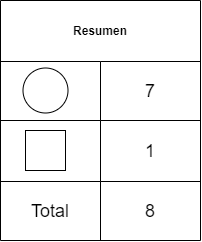
\includegraphics[width=6cm, height=8cm]{imagenes/cap3/DOPcap3Tabla.drawio.png} & 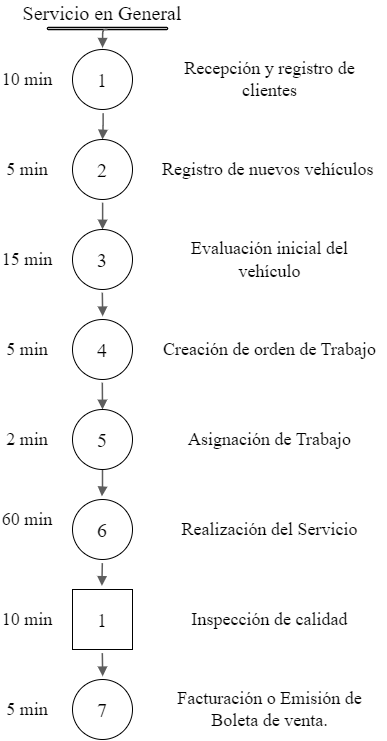
\includegraphics[width=8cm, height=18cm]{imagenes/cap3/DOPCap3.drawio.png} \\
%    \end{tabular}
%    \label{fig:diagramaDOP}
%\end{table}
\begin{figure}[H]
    \caption[Diagrama de Proceos Actual (DOP)]{Diagrama de Procesos Actual (DOP)}
    \centering
    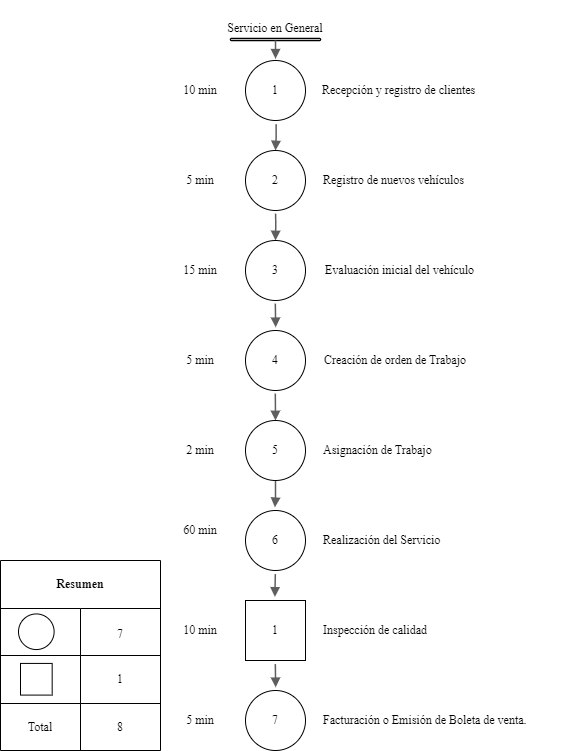
\includegraphics[width=12cm, height=15cm]{imagenes/cap3/DiagramaDOP.drawio.png}
    \label{fig:DiagramaDOP}
\end{figure}


%\begin{table}[H]
%\begin{tabular}{p{5cm}p{22cm}}
% &
% \captionsetup{labelformat=empty}
% \caption{Diagrama DOP}
% \includesvg[width=15cm, height=20cm]{imagenes/cap3/DOP1.svg}
% \label{fig:logo}\cr &
%\end{tabular}
%\end{table}

\subsubsection*{3.1.2 Diagrama de Actividades de Procesos Actual (DAP)}
El diagrama DAP es una herramienta más detallada que permite descomponer las actividades del proceso en pasos específicos y analizar su flujo y secuencia. Proporciona una representación detallada y estructurada de las actividades y decisiones realizadas en cada etapa del proceso de atención al cliente, lo que facilita la identificación de áreas de mejora y la implementación de soluciones efectivas.

\begin{figure}[H]
    \caption[Diagrama de Análisis de Proceso (DAP)]{Diagrama de Análisis de Proceso (DAP)}
    %\includesvg[width=1\textwidth]{imagenes/cap3/}
    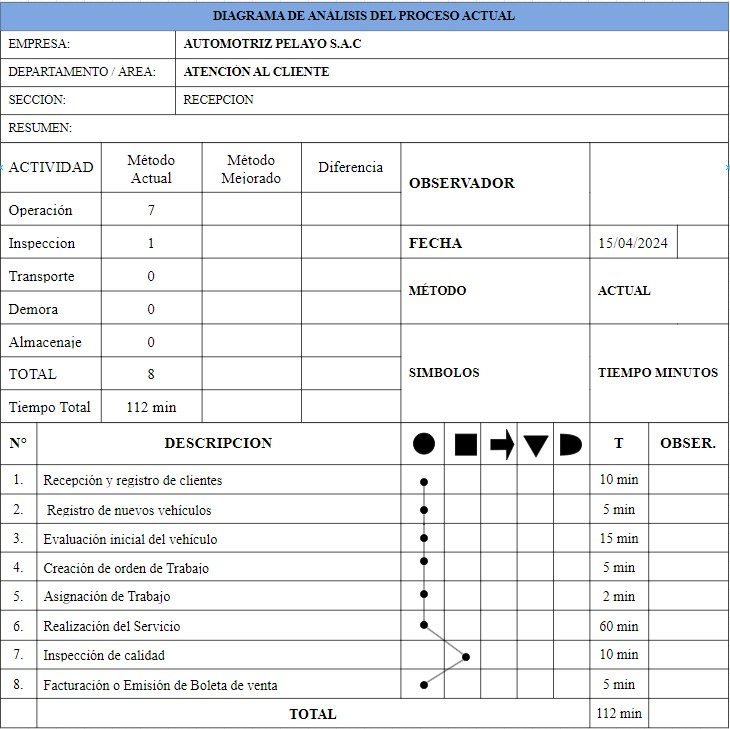
\includegraphics[width=1\textwidth]{imagenes/cap3/DAPcap3captura.jpg}
    %\includegraphics[width=1\textwidth]{imagenes/cap3/DiagramaDOP.png}
    \label{fig:DiagramaDAP}
\end{figure}

\subsection{3.2 Análisis de las causas raíz que generan el problema}
En esta sección del análisis de la situación actual, se procederá a examinar las causas raíz de los problemas detectados en la empresa. Para llevar a cabo este análisis, se utilizará uno de los métodos más reconocidos y utilizados a nivel global en planes de mejora: el método de Ishikawa, también conocido como diagrama de causa-efecto o diagrama de espina de pescado.
\subsubsection*{3.2.1 Método de Ishikawa}
%El Diagrama de Ishikawa es una herramienta visual utilizada para identificar y analizar las posibles causas de un problema específico. En el contexto de este análisis, se aplicará el diagrama de Ishikawa para explorar las diferentes categorías de problemas que afectan el desempeño de la empresa. Cada categoría en el diagrama representa un área potencial de problemas que pueden estar contribuyendo al problema principal, y dentro de cada categoría se identifican las causas específicas.
En el contexto del taller automotriz, se empleará el diagrama de Ishikawa para explorar las diferentes categorías de problemas y sus posibles causas. Cada categoría representa un área potencial de problemas que pueden afectar el desempeño de la empresa. Las escamas principales del diagrama representan estas categorías, mientras que las espinas ramificadas representan las posibles causas dentro de cada categoría.

\begin{enumerate}
    \item Procesos y Procedimientos
    \subsection{Causas:}
    \begin{itemize}
        \item Exceso de tareas en cola: Esto sugiere que hay una acumulación significativa de trabajos pendientes que los operarios deben gestionar, lo cual puede llevar a retrasos y sobrecarga de trabajo.
        \item Gestión de los tiempos de entrega: La ineficaz gestión de los tiempos para completar los trabajos puede resultar en retrasos en la entrega de los vehículos reparados a los clientes.
        \item Retrasos en la facturación: La facturación tardía puede causar problemas de flujo de caja y frustraciones tanto para los clientes como para la empresa.
    \end{itemize}


    \item Infraestructura y Equipamiento
    \subsection{Causas:}
    \begin{itemize}
        \item Infraestructura y equipamiento del taller: Problemas relacionados con la infraestructura física y el equipamiento del taller que podrían afectar la eficiencia y capacidad para manejar la carga de trabajo. Esto puede incluir herramientas obsoletas o en mal estado y una disposición ineficiente del espacio de trabajo.
    \end{itemize}

    \item Recursos Humanos
    \subsection{Causas:}
    \begin{itemize}
        \item Falta de personal capacitado: La carencia de personal con las habilidades y conocimientos necesarios para realizar tareas específicas puede llevar a una disminución en la calidad del servicio y aumentar el tiempo necesario para completar las reparaciones.
        \item Retrasos en la entrega de servicios: La falta de personal adecuado también puede resultar en retrasos en la entrega de los servicios a los clientes.
    \end{itemize}


    \item Materiales y Suministros
    \subsection{Causas:}
    \begin{itemize}
        \item Disponibilidad de piezas y componentes: La falta de disponibilidad de piezas y componentes necesarios para las reparaciones puede resultar en tiempos de espera prolongados para los clientes y afectación en la eficiencia operativa del taller.
    \end{itemize}

    \item Comunicación
    \subsection{Causas:}
    \begin{itemize}
        \item Comunicación con el Cliente: Problemas en la comunicación con los clientes pueden llevar a malentendidos y a una insatisfacción general con el servicio, afectando negativamente la percepción de la empresa.
    \end{itemize}

    \item Gestión de Datos
    \subsection{Causas:}
    \begin{itemize}
        \item Deficiente sistema centralizado de registro: La falta de un sistema eficiente para el registro y gestión de datos puede resultar en duplicidades, errores y dificultades para acceder a información crítica de manera rápida y precisa.
    \end{itemize}

\end{enumerate}

%explicar mejor el diagrama

\begin{landscape}
    \begin{figure}[h]
        \centering
        \caption[Diagrama de Ishikawa]{Diagrama de Ishikawa}
        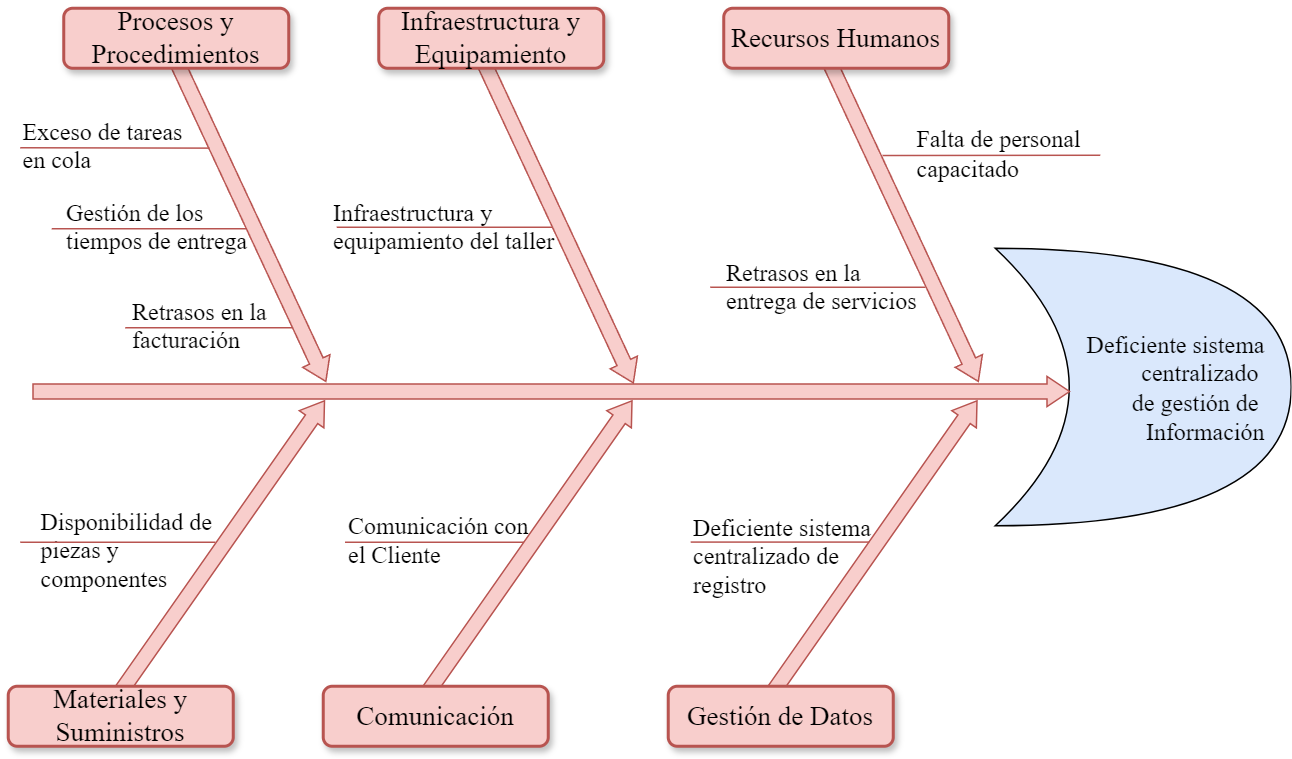
\includegraphics[width=20cm, height=14cm]{imagenes/cap3/IshikawaPescado.drawio.png}
        \label{fig:ishikawa}
    \end{figure}
\end{landscape}

\subsection{3.3 Priorización de causas raíz}
%Se llevó a cabo un análisis detallado de las causas identificadas en el taller, con el objetivo de determinar cuáles tienen el mayor impacto en los problemas observados. Para ello, se utiliza una tabla que muestra la frecuencia de ocurrencia de cada causa raíz y su porcentaje acumulado, lo que permite visualizar de manera clara y concisa cuáles son las principales áreas de mejora.
La priorización de causas raíz es una técnica esencial en la gestión de calidad y resolución de problemas, permitiendo identificar y focalizarse en las causas más significativas que afectan un proceso. En este apartado, se utiliza el Diagrama de Pareto para visualizar y priorizar las causas que generan mayor impacto en el desempeño de un sistema, basándose en el principio de que aproximadamente el 80\% de los problemas son generados por el 20\% de las causas.

\definecolor{ChetwodeBlue}{rgb}{0.556,0.662,0.858}
\begin{table}[H]
\caption[Priorización de causas raíz]{Priorización de causas raíz}
\centering
\begin{tblr}{
  row{1} = {ChetwodeBlue},
  column{1} = {c},
  column{2} = {7.5cm},
  column{3} = {c},
  column{4} = {c},
  column{5} = {c},
  column{6} = {c},
  cell{2}{3} = {c},
  cell{3}{3} = {c},
  cell{4}{3} = {c},
  cell{5}{3} = {c},
  cell{6}{3} = {c},
  cell{7}{3} = {c},
  cell{8}{3} = {c},
  cell{9}{3} = {c},
  cell{10}{3} = {c},
  cell{11}{3} = {c},
  cell{12}{3} = {c},
  hlines,
  vlines,
}
Ítem & Descripcion & Frec & Frec Acum & Porc. & Porc Acum\\
1 & Retrasos
  en la facturación debido al proceso manual y propenso a errores. & 29 & 29 & 25\% & 25\%\\
2 & Deficiente
  sistema centralizado de registro. & 28 & 57 & 24\% & 49\%\\
3 & Dificultades
  para gestionar la demanda en períodos de alta actividad. & 25 & 82 & 21\% & 70\%\\
4 & Exceso
  de tareas en cola para el personal. & 10 & 92 & 9\% & 79\%\\
5 & Deficiencia
  en la gestión de tiempo de los operarios. & 6 & 98 & 5\% & 84\%\\
6 & Deficiencias
  en la infraestructura y equipamiento del taller. & 5 & 103 & 4\% & 88\%\\
7 & Falta
  de personal capacitado para tareas específicas. & 4 & 107 & 3\% & 91\%\\
8 & Retrasos
  en la entrega de servicios. & 5 & 112 & 4\% & 96\%\\
9 & Falta
  de disponibilidad de piezas y componentes necesarios para realizar las
  reparaciones de manera oportuna. & 3 & 115 & 3\% & 98\%\\
10 & Retrasos
  en la entrega de servicios debido a carga de trabajo excesiva & 2 & 117 & 2\% & 100\%\\
 & Total & 117 &  & 100\% & 
\end{tblr}
\end{table}




%La tabla presenta las causas raíz ordenadas según su importancia, destacando aquellas que contribuyen significativamente al total de problemas. Se utiliza el principio de la Ley ABC o Ley 20-80, que sugiere que aproximadamente el 20\% de las causas en estudio generan el 80\% del total de los efectos. En este contexto, se priorizan las causas raíz que representan el 20\% superior en términos de frecuencia de ocurrencia.

%Se elaboro un diagrama de Pareto, para visualizar gráficamente las causas raíz en orden descendente de su frecuencia. Este análisis permite identificar los problemas que requieren mayor atención y desarrollar soluciones inmediatas.

El Diagrama de Pareto presentado, basado en los datos recopilados, permite identificar y priorizar las principales causas raíz de los problemas observados. Este diagrama sigue la regla de Pareto, donde se observa que una pequeña cantidad de causas (aproximadamente el 30\%) contribuye a la mayoría de los efectos (aproximadamente el 70\%).

\begin{figure}[H]
    \caption[Diagrama de Pareto]{Diagrama de Pareto}
    \begin{tabular}{c}
        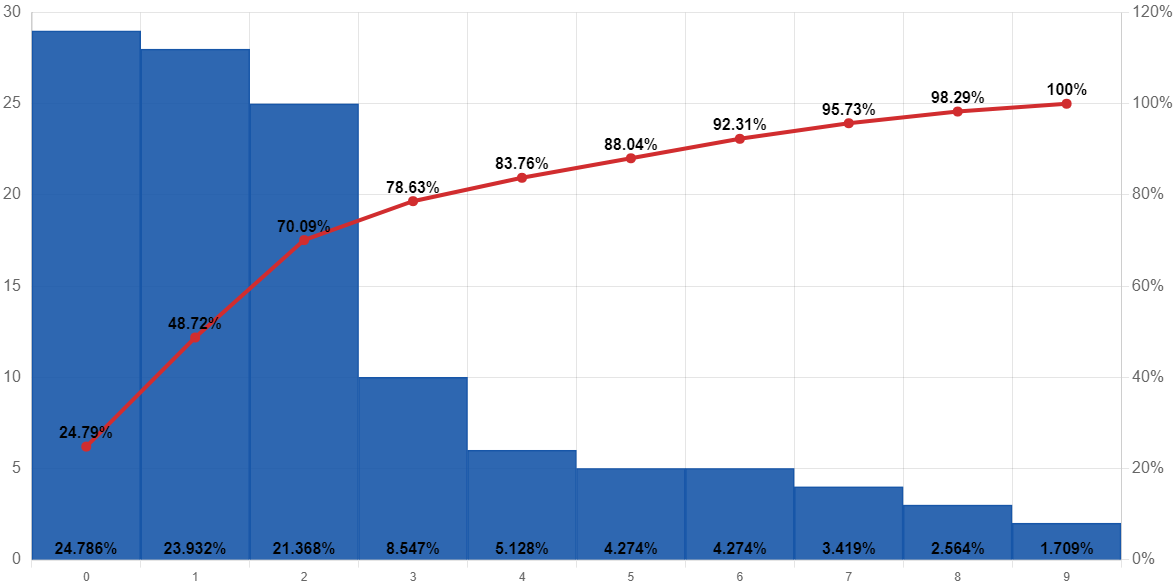
\includegraphics[width=1\textwidth]{imagenes/cap3/diagrama-de-paretoMEj.png}
        %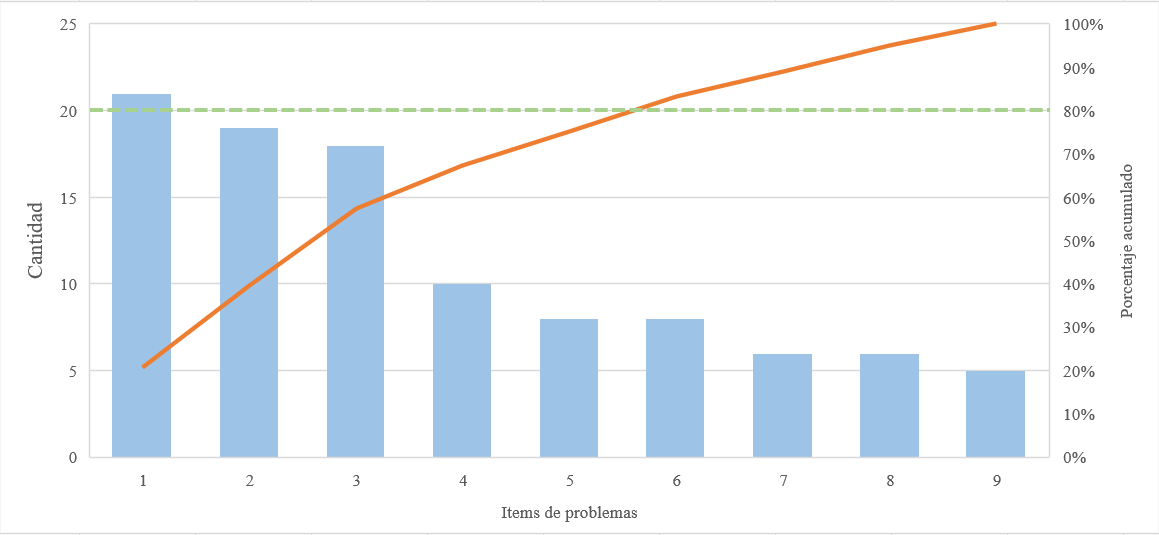
\includegraphics[width=1\textwidth]{imagenes/cap3/Paretov3.png}
    \end{tabular}
    \label{fig:diagramaPareto}
\end{figure}

Como se puede observar en el diagrama, las tres principales causas (retrasos en la facturación, deficiente sistema centralizado de registro y dificultades para gestionar la demanda) contribuyen significativamente a la mayoría de los problemas, acumulando un 70\% de los mismos. Este hallazgo no cumple la regla 80 - 20, pero se acerca y asi se confirma que enfocar los esfuerzos en estas áreas podría resultar en una mejora significativa del sistema general.

%Basado en la información recopilada y los procesos identificados en la empresa antes de la implementación del aplicativo, se observa que existen desafíos significativos en la eficiencia operativa y la gestión de la satisfacción del cliente. Los tiempos de espera prolongados, la falta de coordinación entre los diferentes pasos del servicio y la posible inconsistencia en la calidad del trabajo podrían haber contribuido a una experiencia del cliente insatisfactoria. Además, la falta de una herramienta centralizada para la gestión de los servicios y la comunicación con los clientes podría haber resultado en una falta de seguimiento efectivo y una capacidad limitada para abordar las necesidades específicas de los clientes de manera oportuna. En resumen, el análisis revela áreas clave de mejora que podrían abordarse con la implementación del aplicativo propuesto, con el potencial de optimizar los procesos internos y mejorar la experiencia general del cliente.

%mejorar el diagrama pareto y el diagrama ishikawa.

%-----------CAPITULO 4-----------
\newpage
%Color
\definecolor{ChetwodeBlue}{rgb}{0.556,0.662,0.858}

\section{CAPITULO IV}
\section*{PROPUESTA TÉCNICA DE LA MEJORA}
En este capítulo, se propone una solución técnica para abordar las deficiencias identificadas, con un enfoque en la mejora de los procesos operativos. Se presentan aspectos como la metodología de implementación, recursos técnicos necesarios, cronograma de ejecución y posibles limitaciones que podrían surgir durante el proceso de implementación. A través de la planificación detallada y la asignación de responsabilidades claras, se busca garantizar que la implementación de las mejoras se realice de manera eficiente y efectiva, maximizando los beneficios para la empresa.


\subsection{4.1 Plan de acción de la Mejora propuesta}
%El plan de acción es una herramienta importante en el proceso de implementación de mejoras. Este plan detalla las diversas tareas y actividades necesarias para llevar a cabo la mejora, asignando responsabilidades, recursos y tiempos para cada una de ellas. Esta representado en la tabla 4, constituye un plan que prioriza las iniciativas más importantes para cumplir con los objetivos y/o metas del proyecto. De esta manera, se podrá constituir un plan de acción que nos servirá de guía a la hora de llevar el mismo.

El plan de acción es una herramienta importante en el proceso de implementación de mejoras. Este plan detalla las diversas tareas y actividades necesarias para llevar a cabo la mejora, asignando responsabilidades, recursos y tiempos para cada una de ellas. Representado en la tabla 4, constituye un plan que prioriza las iniciativas más importantes para cumplir con los objetivos y/o metas del proyecto. De esta manera, se podrá constituir un plan de acción que servirá de guía a la hora de llevarlo a cabo.

La tabla 4 proporciona un desglose detallado de las tareas necesarias para implementar una mejora en un sistema de software. Incluye actividades clave como la identificación de requisitos, el diseño y desarrollo de interfaces, la implementación de la arquitectura backend y la integración del frontend y backend. Cada tarea está asignada a un responsable específico y se detallan los recursos necesarios, el tiempo estimado de cada actividad y los indicadores de seguimiento para monitorear el progreso. El plan asegura que cada etapa del proyecto esté bien definida y organizada para facilitar una implementación eficiente y sin problemas en un entorno de producción.

%Diagrama plan de mejora
\begin{landscape}
\begin{table}
\centering
\caption{Plan de acciones de la mejora}
\begin{tblr}{
  cells = {c},
  row{1} = {ChetwodeBlue},
  column{1} = {3.5cm},
  column{2} = {5cm},
  column{3} = {2.2cm},
  column{4} = {0.4cm},
  column{5} = {3cm},
  column{6} = {3.5cm},
  column{7} = {2.8cm},
  cell{2}{3} = {r=2}{},
  cell{2}{7} = {r=9}{},
  cell{7}{3} = {r=2}{},
  cell{7}{5} = {r=3}{},
  vlines,
  hline{1-2,11} = {-}{},
  hline{3} = {1-2,4-6}{},
  hline{4-7,10} = {1-6}{},
  hline{8} = {1-2,4,6}{},
  hline{9} = {1-4,6}{},
}
\textbf{Acciones de Mejora} & \textbf{Tareas} & \textbf{Responsable} & \textbf{T (h)} & \textbf{Recursos Necesarios} & \textbf{Indicador de Seguimiento} & \textbf{Responsable de Seguimiento}\\
Listar requisitos del sistema & Reunión con usuarios para identificar requisitos & Analista de Sistemas & 16 & Hojas & Requisitos & Monitor de empresa\\
Análisis de requisitos & Elaboración de documentación técnica y diagramas &  & 16 & Herramientas de diseño de software & Documentación & \\
Diseño de la interfaz & Creación de prototipos de interfaz & Diseñador UX/UI & 32 & Herramientas de diseño de interfazces & Prototipos aprobados & \\
Desarrollo de la interfaz & Implementación de la interfaz de usuario & Programador & 40 & Entorno de desarrollo & Interfaz funcional. & \\
Diseño de la arquitectura Backend & Definición de la arquitectura usada en el Back-End & Analista de Sistemas & 16 & Herramientas de diseño de software & Arquitectura aprobada & \\
Implementación del Back-end & Codificación de los componentes del sistema & Programador & 64 & Entorno de desarrollo & Sistema Back-End funcional. & \\
Unión del Front-End y Back-End & Codificación de los servicios requeridos para unir ambos lados del sistema &  & 24 &  & Componentes unidos & \\
Pruebas de funciomiento & Verificar que todos los módulos funcionan sin errores & Tester & 24 &  & Módulos funcionando correctamente & \\
Implementación del sistema en entorno de producción & Configuración de servidores y bases de datos & Programador & 24 & Servidores, Bases de datos, AWS & Sistema funcionando correctamente & 
\end{tblr}
\end{table}

\end{landscape}

%\begin{landscape}
%\begin{table}
%\centering
%\captionsetup{labelformat=empty}
%\begin{tblr}{
%  row{1} = {ChetwodeBlue},
%  column{1} = {3.5cm},
%  column{2} = {5cm},
%  column{3} = {2.2cm},
%  column{4} = {0.4cm},
%  column{5} = {3cm},
%  column{6} = {3.5cm},
%  column{7} = {2.8cm},
%  cell{2}{5} = {r=2}{},
%  cell{2}{7} = {r=3}{},
%  vlines,
%  hline{1-2,5} = {-}{},
%  hline{3} = {1-4,6}{},
%  hline{4} = {1-6}{},
%}
%\textbf{Acciones de Mejora} & \textbf{Tareas} & \textbf{Responsable} & \textbf{T (h)} & \textbf{Recursos Necesarios} & \textbf{Indicador de Seguimiento} & \textbf{Responsable de Seguimiento}\\
%Unión del Front-End y Back-End & Codificación de los servicios requeridos para unir ambos lados del sistema & Programador & 24 & Entorno de desarrollo & Componentes unidos & Monitor de empresa\\
%Pruebas de funciomiento & Verificar que todos los módulos funcionan sin errores & Tester & 24 &  & Módulos funcionando correctamente & \\
%Implementación del sistema en entorno de producción & Configuración de servidores y bases de datos & Programador & 24 & Servidores, Bases de datos, AWS & Sistema funcionando correctamente & 
%\end{tblr}
%\end{table}


%\captionsetup{labelformat=empty}
%\begin{longtable}{|p{3.5cm}|p{5cm}|p{2.2cm}|p{0.4cm}|p{3cm}|p{3.5cm}|p{2.8cm}|}
%%\caption[Plan de acciones de la mejora]{\textbf{Plan de acciones de la mejora}}\\
%\hline
%\rowcolor[rgb]{0.557,0.663,0.859} \textbf{Acciones de Mejora} & \textbf{Tareas} & \textbf{Responsable} & \textbf{T (h)} & \textbf{Recursos Necesarios} & \textbf{Indicador de Seguimiento} & \textbf{Responsable de Seguimiento} \endfirsthead 
%\hline
%Unión del Front-End y Back-End & Codificación de los servicios requeridos para unir ambos lados del sistema & Programador & 24 & Entorno de desarrollo & Ambos sistemas unidos correctamente & Monitor de empresa \\ 
%\hline
%Pruebas de funciomiento & Verificar que todos los módulos funcionan sin errores & Tester & 24 & Entorno de desarrollo & Módulos del sistema funcionando correctamente & Monitor de empresa \\ 
%\hline
%Implementación del sistema en entorno de producción & Configuración de servidores y bases de datos & Programador & 24 & Servidores, Bases de datos, AWS & Sistema funcionando correctamente en un entorno de producción & Monitor de empresa \\
%\hline
%\end{longtable}
%\end{landscape}



\subsection{4.2 Consideraciones técnicas para la implementación de la mejora}
En esta sección se detallan los aspectos técnicos que han sido considerados para la implementación de la mejora en el sistema de gestión del taller mecánico. La implementación exitosa de un sistema de software no solo depende de un buen diseño y programación, sino también de la correcta planificación y consideración de diversos factores técnicos que aseguren un desempeño óptimo y una integración eficaz con la infraestructura existente. A continuación, se presentan las principales consideraciones técnicas, incluyendo las especificaciones del equipo, los diagramas de casos de uso, el diagrama de clases, y el diagrama de implementación, así como una lista de recursos técnicos necesarios para llevar a cabo la mejora propuesta.


\subsubsection*{4.2.1 Consideraciones técnicas.}
Para asegurar que el proceso de desarrollo se lleve a cabo de manera eficiente y efectiva, es crucial considerar las especificaciones técnicas del equipo utilizado. Estas especificaciones incluyen detalles sobre el hardware y software empleados por los desarrolladores, que son fundamentales para garantizar la compatibilidad y el rendimiento adecuado del sistema. En la Diagrama 6, se proporciona una ficha técnica que describe en detalle las características del equipo utilizado durante el desarrollo del sistema. Esta información es esencial para entender las capacidades y limitaciones técnicas con las que se ha trabajado y cómo estas influencian el proceso de desarrollo.

En esta sección, se presentan las consideraciones técnicas que fueron tomadas en cuenta durante la implementación de la mejora. Estas consideraciones incluyen las especificaciones del equipo utilizado por el desarrollador durante el proceso de desarrollo del sistema, estas características son descritas en el diagrama 6.

%Ficha tecnica
\begin{figure}[H]
    \caption{Ficha Técnica}
    \begin{tabular}{c}
        %\includesvg[width=1\textwidth]{imagenes/cap3/DOP1.svg} \\
        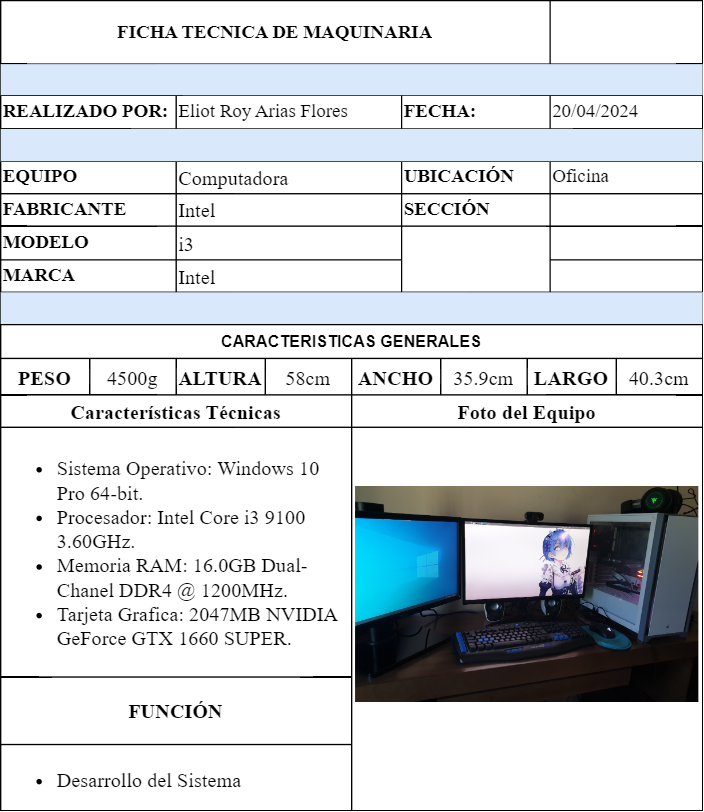
\includegraphics[width=16cm, height=17cm]{imagenes/cap4/FichaTecnica1.png}
    \end{tabular}
    \label{fig:fichaTecnica}
\end{figure}


\subsubsection*{4.2.2 Diagrama de casos de Uso}
El diagrama de casos de uso es una herramienta fundamental dentro de la metodología UML (Unified Modeling Language) que permite visualizar las interacciones entre los usuarios (en este caso, el administrador) y el sistema. Este diagrama ayuda a identificar y organizar las funcionalidades clave del sistema en paquetes específicos, cada uno de los cuales agrupa un conjunto de acciones relacionadas que el usuario puede realizar.

\begin{enumerate}
	\item Gestión de Clientes: Este paquete se encarga de las funcionalidades relacionadas con la gestión de clientes, incluyendo el registro, actualización, búsqueda y eliminación de clientes.
	\begin{itemize}
		\item \textbf{Gestionar Clientes:} Permite al administrador acceder a todas las funcionalidades relacionadas con los clientes.
		\item \textbf{Registrar Cliente:} Permite al administrador registrar un nuevo cliente en el sistema.
		\item \textbf{Actualizar Cliente:} Permite al administrador actualizar la información de un cliente existente en el sistema.
		\item \textbf{Buscar Cliente:} Permite al administrador buscar clientes en la base de datos según ciertos criterios.
		\item \textbf{Eliminar Cliente:} Permite al administrador eliminar un cliente del sistema.
		\item \textbf{Validar Datos:} Verifica que los datos ingresados o actualizados del cliente sean válidos y completos.
	\end{itemize}
	\begin{figure}[H]
		\centering
		\caption{Gestión de Clientes}
		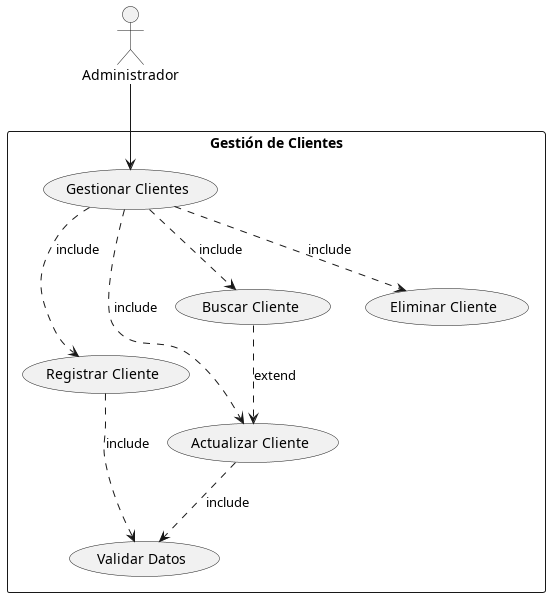
\includegraphics[width=12cm, height=8cm]{imagenes/cap4/casosUso/GestionClientes.png}
		\label{fig:Caso1}
	\end{figure}
	
	\item Gestión de Vehículos: Este paquete se enfoca en las funcionalidades relacionadas con la gestión de vehículos, incluyendo el registro, actualización, búsqueda y eliminación de vehículos.
	\begin{itemize}
		\item \textbf{Gestionar Vehículos:} Permite al administrador acceder a todas las funcionalidades relacionadas con los vehículos.
		\item \textbf{Registrar Vehículo:} Permite al administrador registrar un nuevo vehículo en el sistema.
		\item \textbf{Actualizar Vehículo:} Permite al administrador actualizar la información de un vehículo registrado en el sistema.
		\item \textbf{Buscar Vehículo:} Permite al administrador buscar vehículos en la base de datos según ciertos criterios.
		\item \textbf{Eliminar Vehículo:} Permite al administrador eliminar un vehículo del sistema.
		\item \textbf{Ver Detalles del Vehículo:} Permite al administrador obtener detalles específicos de un vehículo registrado en el sistema.
		\item \textbf{Asociar Vehículo a Cliente:} Permite al administrador vincular un vehículo con su propietario en el sistema.
	\end{itemize}
	\begin{figure}[H]
		\centering
		\caption{Gestión de Vehículos}
		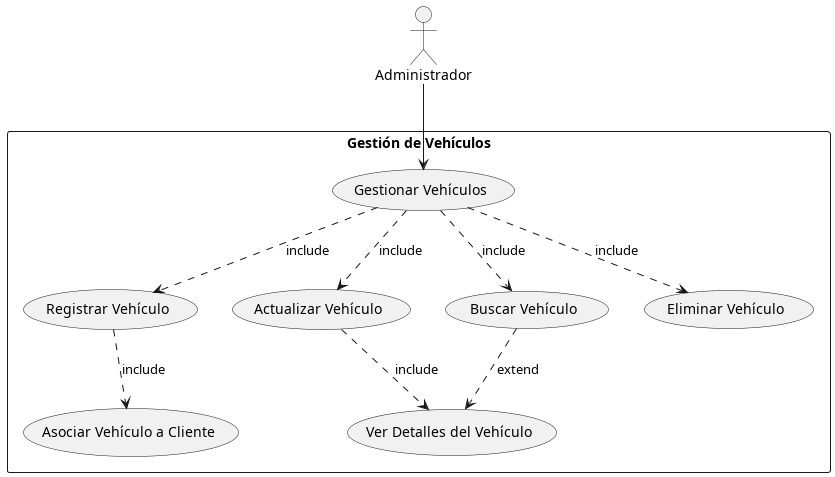
\includegraphics[width=12cm, height=7cm]{imagenes/cap4/casosUso/GestionVehiculos.png}
		\label{fig:Caso2}
	\end{figure}    
	
	\item Gestión de Servicios: Este paquete se dedica a las funcionalidades relacionadas con la gestión de servicios ofrecidos por el taller, incluyendo el registro, actualización, búsqueda y eliminación de servicios.
	\begin{itemize}
		\item \textbf{Gestionar Servicios:} Permite al administrador acceder a todas las funcionalidades relacionadas con los servicios.
		\item \textbf{Registrar Servicio:} Permite al administrador registrar un nuevo servicio en el sistema.
		\item \textbf{Actualizar Servicio:} Permite al administrador actualizar la información de un servicio existente.
		\item \textbf{Buscar Servicio:} Permite al administrador buscar servicios en la base de datos según ciertos criterios.
		\item \textbf{Eliminar Servicio:} Permite al administrador eliminar un servicio del sistema.
		\item \textbf{Asignar Precio:} Permite al administrador establecer o modificar el precio de un servicio.
		\item \textbf{Categorizar Servicio:} Permite al administrador asignar una categoría a un servicio para su mejor organización.
	\end{itemize}
	\begin{figure}[H]
		\centering
		\caption{Gestión de Servicios}
		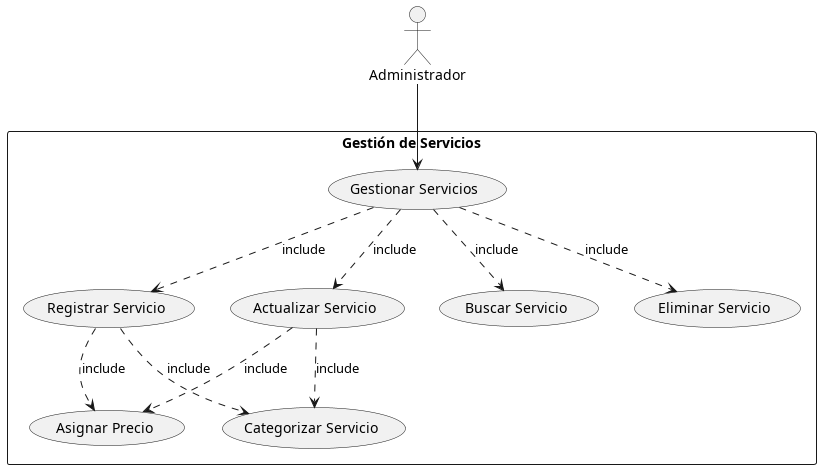
\includegraphics[width=12cm, height=8cm]{imagenes/cap4/casosUso/GestionServicios.png}
		\label{fig:Caso3}
	\end{figure}
	
	\item Gestión de Trabajos:
	Este paquete se encarga de la gestión de las órdenes de trabajo en el taller, abarcando desde el registro de nuevas órdenes hasta su seguimiento y actualización.
	\begin{itemize}
		\item \textbf{Gestionar Trabajos:} Permite al administrador acceder a todas las funcionalidades relacionadas con los trabajos y órdenes.
		\item \textbf{Registrar Orden:} Permite al administrador registrar una nueva orden de trabajo en el sistema.
		\item \textbf{Actualizar Orden:} Permite al administrador actualizar la información de una orden de trabajo existente.
		\item \textbf{Buscar Orden:} Permite al administrador buscar órdenes de trabajo en la base de datos según ciertos criterios.
		\item \textbf{Seguimiento de Orden:} Permite al administrador realizar el seguimiento del estado de una orden de trabajo.
		\item \textbf{Asignar Trabajo a Técnico:} Permite al administrador asignar una orden de trabajo a un técnico específico.
		\item \textbf{Cerrar Orden:} Permite al administrador finalizar una orden de trabajo una vez completada.
	\end{itemize}
	\begin{figure}[H]
		\centering
		\caption{Gestión de Trabajos}
		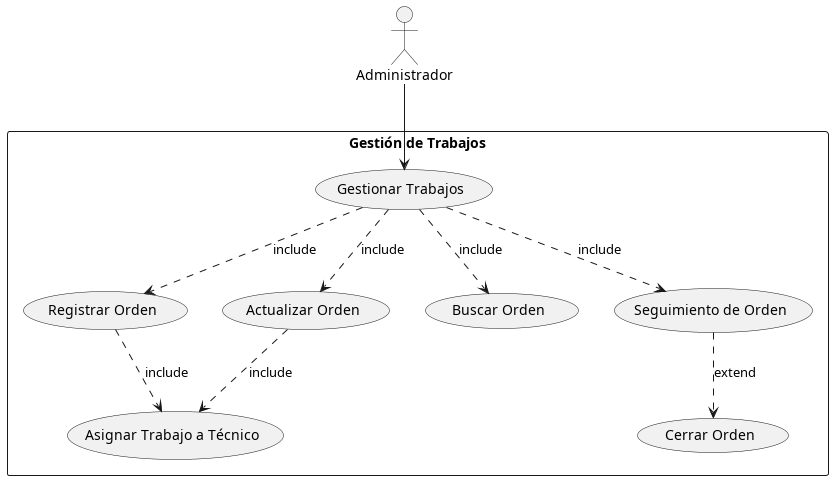
\includegraphics[width=12cm, height=10cm]{imagenes/cap4/casosUso/GestionTrabajos.png}
		\label{fig:Caso4}
	\end{figure}
	
	\item Gestión de Técnicos:
	Este paquete gestiona la información relacionada con los técnicos del taller, incluyendo el registro, actualización, búsqueda y eliminación de técnicos.
	\begin{itemize}
		\item \textbf{Gestionar Técnicos:} Permite al administrador acceder a todas las funcionalidades relacionadas con los técnicos.
		\item \textbf{Registrar Técnico:} Permite al administrador registrar un nuevo técnico en el sistema.
		\item \textbf{Actualizar Técnico:} Permite al administrador actualizar la información de un técnico existente en el sistema.
		\item \textbf{Buscar Técnico:} Permite al administrador buscar técnicos en la base de datos según ciertos criterios.
		\item \textbf{Eliminar Técnico:} Permite al administrador eliminar un técnico del sistema.
		\item \textbf{Ver Detalles del Técnico:} Permite al administrador obtener detalles específicos de un técnico registrado en el sistema.
		\item \textbf{Asignar Especialidad:} Permite al administrador asignar o modificar la especialidad de un técnico.
	\end{itemize}  
	\begin{figure}[H]
		\centering
		\caption{Gestión de Técnicos}
		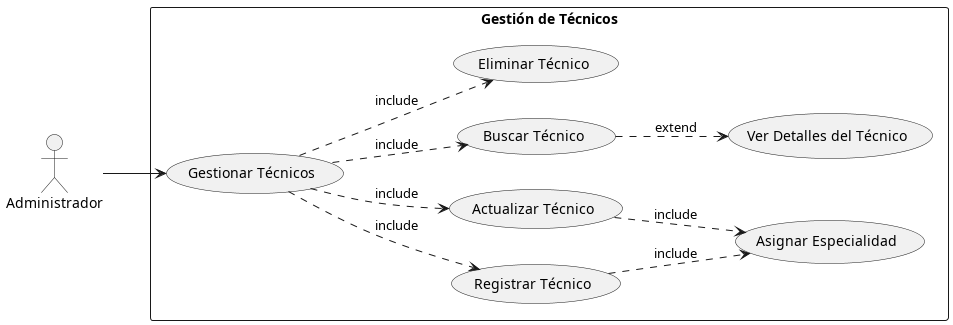
\includegraphics[width=12cm, height=8cm]{imagenes/cap4/casosUso/GestionTecnicos.png}
		\label{fig:Caso5}
	\end{figure}   
	
	\item Facturación:
	Este paquete maneja todas las funcionalidades relacionadas con la facturación de los servicios proporcionados, incluyendo el registro de costos, la generación de facturas y la gestión de los tipos de pago.
	\begin{itemize}
		\item \textbf{Gestionar Facturación:} Permite al administrador acceder a todas las funcionalidades relacionadas con la facturación.
		\item \textbf{Registrar Costos:} Permite al administrador registrar los costos asociados a los servicios realizados.
		\item \textbf{Generar Factura:} Permite al administrador generar una factura para los servicios prestados.
		\item \textbf{Procesar Pago:} Permite al administrador procesar el pago de una factura.
		\item \textbf{Pago con Tarjeta:} Permite al administrador gestionar pagos realizados con tarjeta.
		\item \textbf{Pago en Efectivo:} Permite al administrador gestionar pagos realizados en efectivo.
		\item \textbf{Anular Factura:} Permite al administrador anular una factura en caso de ser necesario.
	\end{itemize}
	\begin{figure}[H]
		\centering
		\caption{Facturación}
		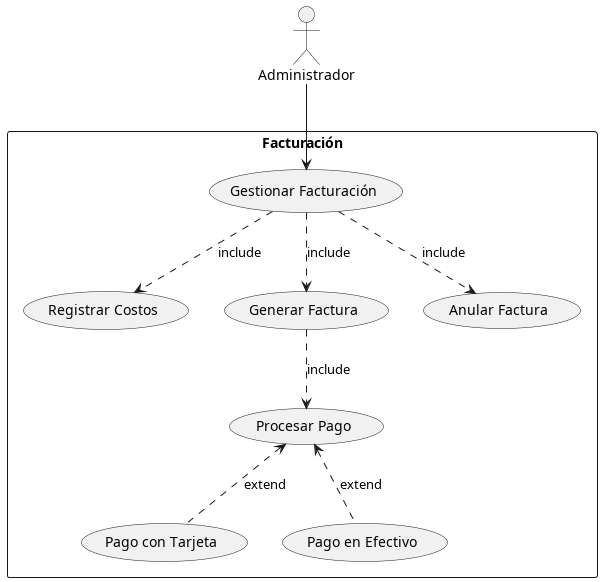
\includegraphics[width=12cm, height=9cm]{imagenes/cap4/casosUso/Facturacion.png}
		\label{fig:Caso6}
	\end{figure}      
	
	\item Reportes y Estadísticas:
	Este paquete se enfoca en la generación de reportes y la recopilación de estadísticas sobre los servicios proporcionados por el taller.
	\begin{itemize}
		\item \textbf{Gestionar Reportes:} Permite al administrador acceder a todas las funcionalidades relacionadas con reportes y estadísticas.
		\item \textbf{Generar Reporte de Ventas:} Permite al administrador generar un reporte detallado de las ventas realizadas.
		\item \textbf{Generar Reporte de Servicios:} Permite al administrador generar un reporte sobre los servicios prestados.
		\item \textbf{Ver Estadísticas:} Permite al administrador visualizar estadísticas generales sobre el rendimiento del taller.
		\item \textbf{Exportar Reportes:} Permite al administrador exportar los reportes generados en diferentes formatos.
		\item \textbf{Personalizar Reporte:} Permite al administrador ajustar los parámetros de los reportes según sus necesidades.
	\end{itemize}  
	\begin{figure}[H]
		\centering
		\caption{Reportes y Estadísticas}
		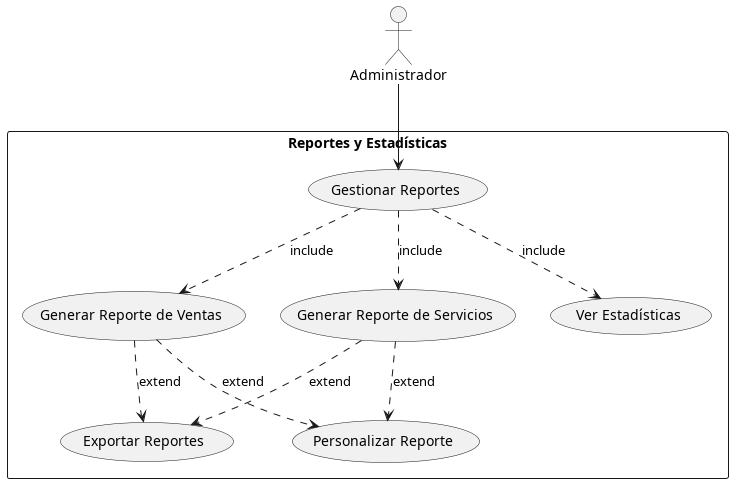
\includegraphics[width=12cm, height=8cm]{imagenes/cap4/casosUso/ReportesEstadisticas.png}
		\label{fig:Caso7}
	\end{figure}     
\end{enumerate}


\subsubsection*{4.2.3 Diagrama de clases}
%El diagrama de clases  en un representación visual de la estructura estática del sistema, muestra las clases, sus atributos y la forma en la que interactúan entre ellas. Este diagrama es útil para comprender la organización de los datos y las entidades del sistema. cada clase representa un conjunto de objetos con características similares, como usuario, clientes, vehículos, servicios, entre otros. Este diagrama forma parte del diseño para la implementación del sistema, permitiendo una mejor comprensión de su funcionamiento. Se puede ver en la pagina \pageref{fig:Dclases}

El diagrama de clases es una representación visual de la estructura estática del sistema, mostrando las clases, sus atributos y las relaciones entre ellas. Este diagrama es esencial para comprender la organización de los datos y las entidades que forman parte del sistema. Cada clase representa un conjunto de objetos con características similares, como usuarios, clientes, vehículos, servicios, entre otros. El diagrama de clases es una herramienta crucial en el diseño del sistema, ya que proporciona una visión detallada de la estructura del mismo, facilitando su implementación y asegurando una coherencia en la representación de los datos.

\subsubsection*{Descripción General}
\begin{enumerate}
    \item Cliente: Representa a los clientes, incluyendo su información de contacto y tipo de pago. Un cliente puede tener múltiples vehículos asociados.
    \item Vehículo: Registra los vehículos, con detalles como marca y modelo. Cada vehículo está vinculado a un cliente y puede tener múltiples órdenes de trabajo.
    \item Técnico: Describe a los técnicos del taller, con su especialidad y estado laboral. Cada técnico puede estar asignado a varias órdenes de trabajo.
    \item Servicios: Define los servicios que ofrece el taller, incluyendo el costo y la duración estimada. Los servicios son utilizados en las órdenes de trabajo.
    \item OrdenTrabajo: Gestiona las órdenes de trabajo para los vehículos, incluyendo los servicios realizados y el técnico asignado. Se registra la fecha de ingreso y salida del vehículo y el estado de la orden.
    \item Factura: Genera facturas vinculadas a un cliente, un vehículo y una orden de trabajo específica.
\end{enumerate}

\subsubsection*{Relaciones Clave}
\begin{itemize}
    \item Cliente-Vehículo: Un cliente puede poseer múltiples vehículos.
    \item Vehículo-OrdenTrabajo: Un vehículo puede tener varias órdenes de trabajo.
    \item OrdenTrabajo-Servicios: Una orden de trabajo puede incluir varios servicios.
    \item OrdenTrabajo-Técnico: Cada orden es atendida por un técnico específico.
    \item Factura: Relaciona un cliente, vehículo y orden de trabajo con una factura.    
\end{itemize}

%Diagrama de clases 
\begin{landscape}
    \begin{figure}
        \caption{Diagrama de clases}
        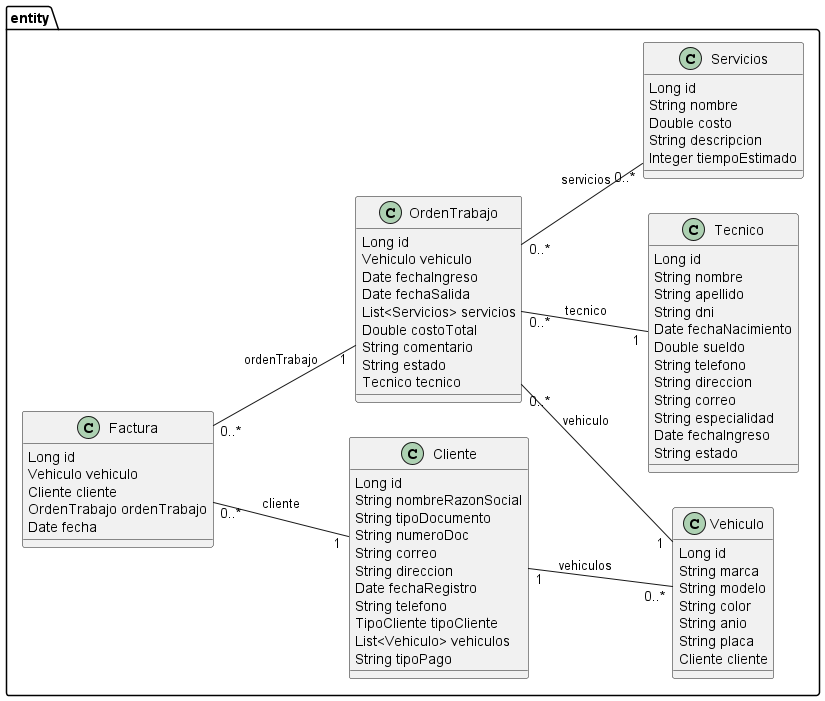
\includegraphics[width=22cm, height=16cm]{imagenes/cap4/ClaseInfoEntidad.png}
        \label{fig:Dclases}
    \end{figure}
\end{landscape}


\subsubsection*{4.2.4 Diagrama de Implementación}
Este diagrama es una representación visual de como se despliegan físicamente los componentes del sistema, incluyendo hardware y software, y cómo se comunican entre sí. Aquí se muestran los nodos físicos y las conexiones entre ellos, lo que ayuda a comprender la distribución de los diferentes elementos del sistema en el entorno de implementación. Es útil al planificar la infraestructura necesaria y asegurar una correcta implementación del sistema.

%\begin{landscape}
    \begin{figure}[H]
    \centering
    \caption[Diagrama de Implementación]{Diagrama de Implementación}
    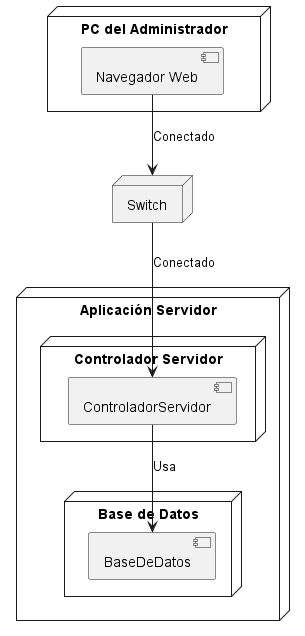
\includegraphics[width=8cm, height=15cm]{imagenes/cap4/diagramaImplementacion.png}
    \label{fig:DIMplementacion}
    \end{figure}
%\end{landscape}


\subsection{4.3 Recursos técnicos para implementar la mejora propuesta}
En esta sección, se detallan los recursos técnicos necesarios para llevar a cabo la implementación de la mejora propuesta. Se presentan los equipos, materiales, recursos humanos y documentación requeridos para el desarrollo y puesta en marcha del sistema. Cada tabla proporciona información sobre el tipo y cantidad de recursos necesarios, lo que permitirá una planificación más precisa y eficiente de los recursos disponibles para el proyecto. Esta fase es fundamental para asegurar que se cuenta con los medios adecuados para llevar a cabo la mejora de manera efectiva.

\begin{table}[H]
\centering
\caption{Equipos}
\label{tab:Equipos}
\begin{tblr}{
  cells = {c},
  row{1} = {ChetwodeBlue},
  rowsep = 3pt,
  hlines,
  vlines,
}
\textbf{Equipos} & \textbf{ Detalles}\\
Computadora & 1\\
Internet & 1
\end{tblr}
\end{table}

%\subsubsection*{Materiales}
\begin{table}[H]
\centering
\caption{Materiales}
\label{tab:Equipos}
\begin{tblr}{
  cells = {c},
  row{1} = {ChetwodeBlue},
  rowsep = 3pt,
  hlines,
  vlines,
}
\textbf{Software} & \textbf{ Detalles}\\
Lenguajes de Programación & 3\\
Base de datos & 1\\
Software de desarrollo & 1\\
Software de diseño & 1
\end{tblr}
\end{table}

%\subsubsection*{Recursos Humanos}
\begin{table}[H]
\centering
\caption{Recursos Humanos}
\label{tab:Equipos}
\begin{tblr}{
  cells = {c},
  row{1} = {ChetwodeBlue},
  rowsep = 3pt,
  hlines,
  vlines,
}
\textbf{Recursos Humanos} & \textbf{ Detalles}\\
Analista de Sistemas & 32 horas\\
Arquitecto de Software & 16 horas\\
Diseñador UX/UI & 32 horas\\
Desarrollador Front-End & 40 horas\\
Desarrollador Back-End & 64 horas\\
Tester & 24 horas
\end{tblr}
\end{table}



%\subsubsection*{Documentación}
\begin{table}[H]
\centering
\caption{Documentación}
\label{tab:Equipos}
\begin{tblr}{
  cells = {c},
  row{1} = {ChetwodeBlue},
  rowsep = 3pt,
  hlines,
  vlines,
}
\textbf{Documentación} & \textbf{ Detalles}\\
Lista de Requerimientos & 1\\
Documentación del Proyecto & 1
\end{tblr}
\end{table}


\subsection{4.4 Diagrama del proceso, mapa del flujo de valor y/o diagrama de operación de la situación mejorada}
En esta sección se presentara el diagrama de análisis de proceso mejorados, este diagrama reflejara los procesos mejorados y optimizados, considerando que el sistema de mejora ha sido implementado con éxito. Además, se destacarán los beneficios obtenidos a partir de estas mejoras, lo que permitirá visualizar claramente el impacto positivo en la eficiencia de los servicios ofrecidos.\\
En el diagrama 16 se puede ver la diferencia entre los tiempos de atención antes y después de la implementación de la mejora, ahorrando a la empresa 18 minutos durante cada servicio ofrecido.

\begin{figure}[H]
    \caption{Diagrama de Análisis de Proceso Mejorado}
    \begin{tabular}{c}
        %\includesvg[width=17cm, height=19cm]{imagenes/cap4/DAPmejorado.drawio.svg} \\
        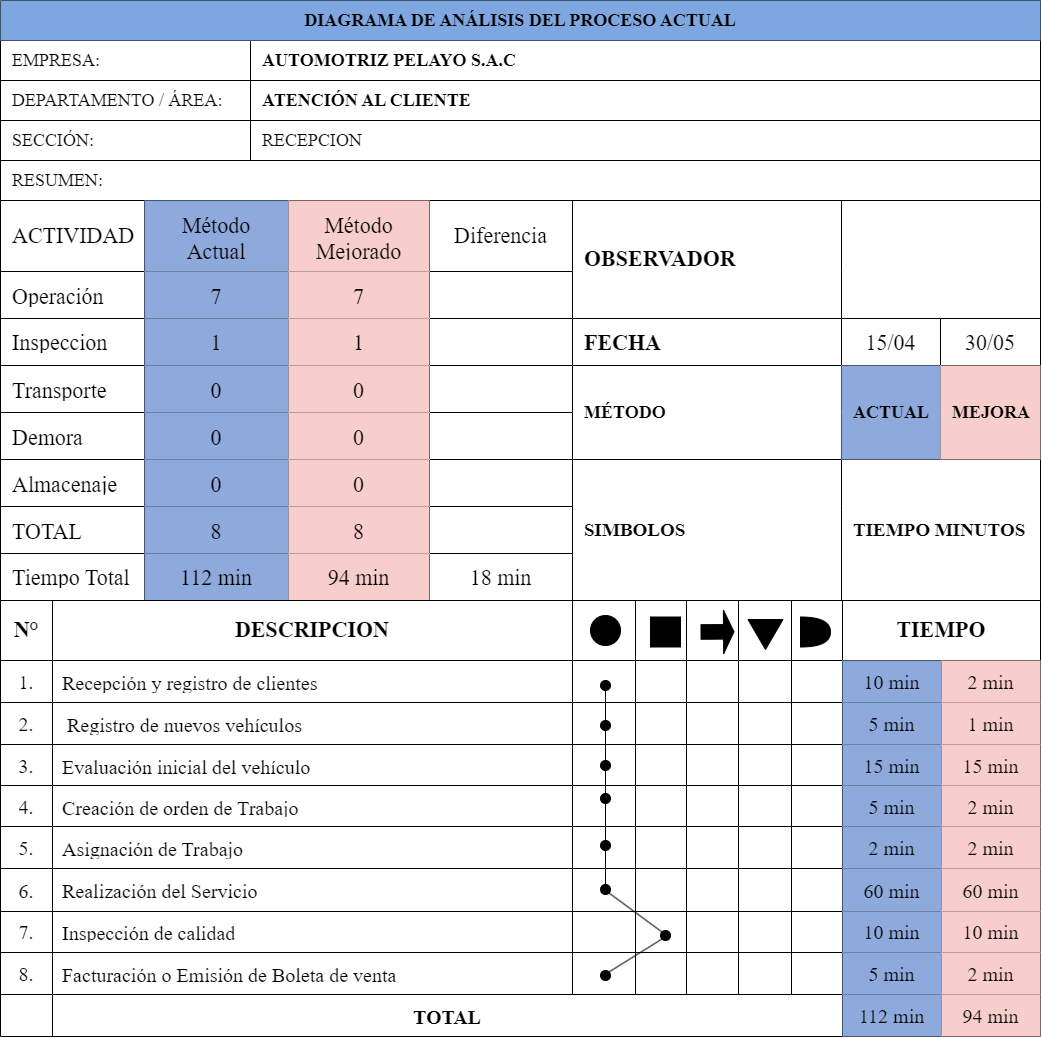
\includegraphics[width=16cm, height=18cm]{imagenes/cap4/DAPmejoradov2.drawio.png}
    \end{tabular}
    \label{fig:DAPMejorado}
\end{figure}


\subsection{4.5 Cronograma de ejecución de la mejora}
En esta sección se detalla el cronograma de ejecución de la mejora propuesta, donde se establece el orden en que se desarrollarán las actividades necesarias para llevar a cabo la implementación del proyecto de mejora. Cada actividad tiene asignado un responsable específico, como se muestra en la tabla 10. Este cronograma proporciona una visión general del tiempo requerido para cada tarea. Además, sirve como herramienta para detectar posibles retrasos en el cumplimiento de los plazos y actuar de inmediato.

\begin{table}[H]
\centering
\caption{Cronograma de ejecución de la mejora}
\label{tab:Cronograma}
\begin{tblr}{
  row{1} = {ChetwodeBlue},
  column{1} = {7cm},
  cell{1}{1} = {c},
  cell{2}{2} = {blue,c},
  cell{3}{3} = {blue,c},
  cell{4}{4} = {blue,c},
  cell{4}{5} = {c},
  cell{5}{5} = {blue,c},
  cell{5}{6} = {blue,c},
  cell{6}{6} = {blue},
  cell{6}{7} = {blue,c},
  cell{6}{8} = {c},
  cell{7}{7} = {blue},
  cell{7}{8} = {blue,c},
  cell{7}{9} = {c},
  cell{8}{8} = {blue},
  cell{8}{10} = {c},
  cell{9}{9} = {blue},
  cell{9}{10} = {blue},
  cell{9}{11} = {c},
  cell{10}{11} = {blue,c},
  hlines,
  vlines,
}
\textbf{Tiempo de Ejecución} & \textbf{S1} & \textbf{S2} & \textbf{S3} & \textbf{S4} & \textbf{S5} & \textbf{S6} & \textbf{S7} & \textbf{S8} & \textbf{S9} & \textbf{S10}\\
Listar
  requisitos del sistema &  &  &  &  &  &  &  &  &  & \\
Análisis
  de requisitos &  &  &  &  &  &  &  &  &  & \\
Diseño
  de la interfaz &  &  &  &  &  &  &  &  &  & \\
Desarrollo
  de la interfaz &  &  &  &  &  &  &  &  &  & \\
Diseño
  de la arquitectura Backend &  &  &  &  &  &  &  &  &  & \\
Implementación
  del Back-End &  &  &  &  &  &  &  &  &  & \\
Unión
  del Front-End y Back-End &  &  &  &  &  &  &  &  &  & \\
Pruebas
  de funcionamiento &  &  &  &  &  &  &  &  &  & \\
Implementación del sistema en entorno de
  producción &  &  &  &  &  &  &  &  &  & 
\end{tblr}
\end{table}


\subsection{4.6 Aspectos limitantes para la implementación de la mejora}
En esta sección se abordara las limitaciones o dificultades que surgen durante la implementación de la acción de mejora pueden ser un factor clave a tomar en cuenta, puesto que pueden llegar a determinar la consecución, o no del proyecto. Algunas de las dificultades que surgieron la implementación fueron las siguientes:
\begin{enumerate}
    \item Recursos financieros limitados: La disponibilidad de fondos puede ser un factor restrictivo, ya que algunas mejoras pueden requerir una inversión significativa en tecnología, capacitación de personal o infraestructura.
    \item Resistencia al cambio: El cambio puede enfrentar resistencia por parte de los empleados que están acostumbrados a los procesos antiguos o temen la pérdida de control sobre su trabajo.
    \item Factor de Tiempo: Algunos plazos ajustados pueden dificultar el cumplimiento adecuado de todas las etapas del proyecto. Esto puede llevar a la necesidad de priorizar ciertas actividades sobre otras o comprometer la calidad del trabajo realizado.
    \item Limitaciones técnicas: Pueden surgir desafíos técnicos durante la implementación, como problemas de compatibilidad entre diferentes sistemas. Esta complejidad técnica puede ralentizar el progreso del proyecto y requerir soluciones rápidas para superar los obstáculos.
\end{enumerate}
\begin{table}[H]
\centering
\caption{Diagrama de Limitaciones}
\label{tab:Equipos}
\begin{tblr}{
  column{1} = {wd=1cm},
  column{2} = {wd=5.4cm},
  column{3} = {wd=8.9cm},
  row{1} = {ChetwodeBlue,c},
  cell{2}{1} = {c},
  cell{3}{1} = {c},
  cell{4}{1} = {c},
  cell{5}{1} = {c},
  hlines,
  vlines,
}
\textbf{Ítem} & \textbf{Aspecto Observado} & \textbf{Indicador}\\
01 & Recursos financieros limitados & Disponibilidad limitada de fondos para inversión\\
02 & Resistencia al cambio & Actitudes negativas hacia la implementación de mejoras\\
03 & Factor de tiempo & Plazos ajustados para cumplir con todas las etapas del proyecto\\
04 & Limitaciones técnicas & Problemas de compatibilidad entre sistemas o tecnologías
\end{tblr}
\end{table}








%Diagrama de Ganttt
%\begin{landscape}
%    \hspace{3cm}
%    \begin{table}[h]
%    \captionsetup{labelformat=empty}
%    \caption[Diagrama de Gantt]{\textbf{Diagrama de Gantt realizado en GanntProyect}}
%    \begin{tabular}{c}
%        \includegraphics[width=22cm, height=10cm]{imagenes/cap4/DiagramaGant1.jpg}
%    \end{tabular}    
%    \label{fig:DiagramaGant}
%\end{table}
%\end{landscape}


%cuidar el pie de pagina.. 
%referencianr por el numero de diagrama o grafico
%la imagen del los casos de uso deben ser del mismo tamaño
%-----------CAPITULO 5-----------
\newpage
\section{CAPITULO V}
\section*{COSTOS DE IMPLEMENTACIÓN DE LA MEJORA}
%Introducción
Este capitulo se centra en el análisis detallado de los costos de la implementación de la mejora. A través de cada punto, se examinaran los costos materiales, mano de obra, equipos entre otros gastos relevantes para la ejecución del proyecto. El objetivo es proporcionar una visión completa de los recursos financieros necesarios para llevar a cabo la mejora con éxito.

\subsection{5.1 Costo de materiales}
%Introducción
En esta sección, se detallan los costos asociados con los materiales necesarios para la implementación de la mejora propuesta. 
\definecolor{ChetwodeBlue}{rgb}{0.556,0.662,0.858}
\begin{table}[H]
\centering
\caption{Costos de materiales}
\begin{tblr}{
  cells = {c},
  row{1} = {ChetwodeBlue},
  vline{-} = {1-5}{},
  vline{4-6} = {6}{},
  hline{1-6} = {-}{},
  hline{7} = {4-5}{},
}
\textbf{Ítem} & \textbf{Descripción} & \textbf{~Cantidad} & \textbf{Costo Unitario} & \textbf{Monto Total}\\
1 & Lapicero & 2 & ~S/. 1.00 & ~S/. 2.00\\
2 & Hojas Bond & 50 & ~S/. 0.10 & ~S/. 5.00\\
3 & Lapiz & 1 & ~S/. 0.50 & ~S/. 0.50\\
4 & Borrador & 1 & ~S/. 1.00 & ~S/. 1.00\\
 &  &  & ~Total~ & ~S/. 8.50
\end{tblr}
\label{tab:costoMateriales}
\end{table}
En la tabla \ref{tab:costoMateriales} se detallaron los costos de materiales identificados para la implementación de la mejora propuesta. Se han incluido ítems como lapiceros, hojas bond, lápices y borradores, junto con su respectiva cantidad y costo unitario. El monto total representa la suma de todos los gastos. Estos costos son útiles para la planificación financiera y asegurar la disponibilidad de los recursos necesarios.  

\subsection{5.2 Costo de Recursos Humanos}
%Introducción
Estos costos se definen como el esfuerzo de carácter físico y mental que un trabajador realiza a cambio de dinero. Es el personal que posee toda organización para llevar a cabo sus actividades empresariales. En este apartado se detallan los costos asociados con el trabajo realizado por el personal involucrado en la implementación de la mejora propuesta.

\subsubsection*{Desglose de Cálculos}
\begin{enumerate}
    \item Analista de Sistemas:
    \begin{itemize}
        \item Sueldo promedio: S/ 2200
        \item Horas trabajadas: 48
        \item Costo por hora: S/ 13.75
        \item Costo total: 48 horas * S/ 13.75/hora = S/ 660.00
    \end{itemize}
    
    
    \item Diseñador de Interfaces:
    \begin{itemize}
        \item Sueldo promedio: S/ 2450
        \item Horas trabajadas: 32
        \item Costo por hora: S/ 15.31
        \item Costo total: 32 horas * S/ 15.31/hora = S/ 489.92
    \end{itemize}
    
    
    \item Programador Fullstack:
    \begin{itemize}
        \item Sueldo promedio: S/ 2900
        \item Horas trabajadas: 152
        \item Costo por hora: S/ 18.13
        \item Costo total: 152 horas * S/ 18.13/hora = S/ 2751.76
    \end{itemize}    
    
    \item Tester:
    \begin{itemize}
        \item Sueldo promedio: S/ 1203
        \item Horas trabajadas: 24
        \item Costo por hora: S/ 7.52
        \item Costo total: 24 horas * S/ 7.52/hora = S/ 180.48
    \end{itemize}
    
\end{enumerate}

\begin{table}
\centering
\caption[Costo de Recursos Humanos]{Costo de Recursos Humanos}
\begin{tblr}{
  cells = {c},
  row{1} = {ChetwodeBlue},
  vline{-} = {1-5}{},
  vline{2-6} = {6}{},
  hline{1-6} = {-}{},
  hline{7} = {2-5}{},
}
\textbf{Ítem} & \textbf{Descripción} & \textbf{Horas - Hombre} & \textbf{Costo Hora} & \textbf{Costo Total}\\
1 & Analista de Sistemas & 48 & S/ 13.8 & S/ 660.0\\
2 & Diseñador Interfaces & 32 & S/ 15.3 & S/
  489.9\\
3 & Programador & 152 & S/ 18.1 & S/ 2,755.8\\
4 & Tester & 24 & S/ 7.5 & S/
  180.5\\
 & Total & 256 &  & S/ 4,086.2
\end{tblr}
\label{tab:costoRH}
\end{table}

La tabla \ref{tab:costoRH} los costos de la mano de obra para la implementación de la mejora propuesta. Se han incluido los roles de analistas, diseñadores de interfaces, programadores y testers junto con la cantidad de horas-hombre dedicadas a cada uno y el costo por hora. \\
El monto total representa la suma de los costos individuales de cada trabajador, obteniendo asi la estimación precisa de los gastos asociados con la mano de obra necesaria para el proyecto. Es importante destacar que el programador genera la mayor inversión debido a su papel fundamental en el desarrollo del proyecto.

\subsection{5.3 Costo de máquinas, herramientas y equipos}
%Introducción
La evaluación de costos relacionados con equipos es importante para presupuestar proyectos de mejora de manera precisa. Este análisis implica el costeo del uso adecuado del equipo para la implementación del trabajo.

\begin{table}[H]
\centering
\caption[Costo de equipos]{Costo de equipos}
\begin{tblr}{
  cells = {c},
  column{2} = {3cm}, 
  row{1} = {ChetwodeBlue},
  vline{-} = {1-2}{},
  vline{5-7} = {3}{},
  hline{1-3} = {-}{},
  hline{4} = {5-6}{},
}
\textbf{Ítem} & \textbf{Uso de máquina} & \textbf{Horas Totales / Mes} & \textbf{Horas Totales} & \textbf{Costo / Hora} & \textbf{Costo Total}\\
1 & {Computadora de
\\~Escritorio} & 128 & 512 & S/ 2.00 & S/ 1,024.00\\
 &  &  &  & Total & S/
  1,024.00
\end{tblr}
\label{tab:costoEquipos}
\end{table}

La tabla \ref{tab:costoEquipos} muestra los costos asociados con el uso del único ítem que se uso durante la implementación de la mejora. El costo total representa la suma de los gastos incurridos por el uso del equipo durante el período definido para el proyecto. 


\subsection{5.4 Otros costos de implementación de la Mejora}
%Introducción
%En esta sección se analizan los costos adicionales igual de relevantes para el proyecto, estos valores son importantes para determinar el costo-beneficio. Se incluyo el aspecto economico del uso de energia que no fue abordado anteriormente.
En esta sección, se analizan los costos adicionales que son igual de relevantes para el proyecto. Estos valores son esenciales para determinar la relación costo-beneficio y asegurar la viabilidad económica de la implementación. Se ha incluido una evaluación detallada del costo de la energía eléctrica consumida, la suscripción a la API de SUNAT, y el servicio de Internet, los cuales son factores clave que no se abordaron en secciones anteriores. La identificación y cuantificación de estos costos son cruciales para una evaluación completa y precisa de los recursos necesarios para llevar a cabo la mejora propuesta.

\begin{table}[H]
\centering
\caption[Costo de servicios]{Costo de servicios}
\begin{tblr}{
  cells = {c},
  row{1} = {ChetwodeBlue},
  vline{-} = {1-4}{},
  vline{5-7} = {5}{},
  hline{1-5} = {-}{},
  hline{6} = {5-6}{},
}
\textbf{Ítem} & \textbf{Descripción} & \textbf{Unidad} & \textbf{Precio Unitario} & \textbf{Cantidad} & \textbf{Costo Total}\\
1 & Api Sunat & - & - & 1 & S/ 50.00\\
1 & Internet & - & - & mensual & S/
  90.00\\
1 & Energía eléctrica & 0.22 & S/ 0.50 & 128 & S/ 14.00\\
 &  &  &  & Total & S/
  154.00
\end{tblr}
\label{tab:costoServicios}
\end{table}

La tabla \ref{tab:costoServicios} detalla los costos de servicios adicionales asociados a la implementación del proyecto. Estos costos incluyen la suscripción a servicios externos necesarios para la operación del sistema y el consumo de recursos energéticos. Cada ítem está desglosado en su unidad correspondiente, precio unitario, cantidad requerida y el costo total asociado. Presenta una vista detallada de los costos estimados relacionados con la implementación del proyecto de mejora. Se incluyen los siguientes elementos:

\begin{itemize}
    \item API SUNAT: El costo de la suscripción anual a la API de SUNAT, necesaria para acceder a información tributaria y cumplir con las normativas fiscales.
    \item Internet: El costo mensual del servicio de Internet, indispensable para la conectividad y el funcionamiento de los sistemas en línea.
    \item Energía eléctrica consumida estimada: El costo asociado al consumo de energía eléctrica durante el desarrollo del proyecto, calculado en kilovatios-hora (kWh). Se ha aplicado un costo promedio de S/ 0.50 por kWh para estimar el consumo total de la computadora a lo largo del período del proyecto.

\end{itemize}


%La tabla muestra el costo estimado de la energía eléctrica consumida durante la implementación del proyecto de mejora. Se ha calculado el consumo estimado en kilovatios-hora(kWh) y se ha aplicado un costo por hora, considerando el valor de kilovatio-hora en Arequipa. En este caso, se estimo el consumo total de energía de la computador durante el tiempo definido del proyecto.

\subsection{5.5 Costo total de la implementación de la Mejora}
%Introducción
Esta sección presenta el resumen de todos los costos propuestos para la implementación de la mejora. Es costo total es un indicativo del valor estimado necesario para ejecutar las mejoras. Conocer estos costos ayudara a comprender la viabilidad económica del proyecto y asi determinar la factibildidad.

\begin{table}[H]
\centering
\caption{Coste Total}
\begin{tblr}{
  cells = {c},
  row{1} = {ChetwodeBlue},
  vline{-} = {1-5}{},
  vline{2-4} = {6}{},
  hline{1-6} = {-}{},
  hline{7} = {2-3}{},
}
\textbf{N°} & \textbf{Descripción} & \textbf{Costo Total}\\
1 & Costo materiales & S/ 8.50\\
2 & Costo de RRHH & S/
  4,086.16\\
3 & Costo de equipos & S/ 1,024.00\\
4 & Coste de servicios & S/
  154.00\\
 & Total & S/ 5,272.66
\end{tblr}
\end{table}

La tabla resume los costos totales considerando los costos de materiales, mano de obra, equipos y el costo de energía eléctrica como componentes principales del presupuesto total, de esta forma se proporciona una vista general del gasto previsto para la mejora.


%-----------CAPITULO 6-----------
\newpage
\section{CAPITULO VI}
\section*{EVALUACIÓN TÉCNICA Y ECONÓMICA DE LA MEJORA}
En este capitulo se evaluará técnica y económicamente la propuesta de mejora para determinar su factibilidad de aplicación. Para ello, se utilizará el método de análisis Costo/Beneficio, el cual es el proceso de monetizar los diferentes costos y beneficios de una actividad. Este análisis permite estimar el impacto financiero acumulado de lo que se desea lograr y evaluar si el proyecto es rentable o no.
La relación costo-beneficio (B/C), también conocida como índice neto de rentabilidad, se obtiene dividiendo el Valor Actual de los Ingresos totales netos o beneficios netos (VAI) entre el Valor Actual de los Costos de inversión o costos totales (VAC) de un proyecto:

\[\frac{Costo}{Beneficio} = \frac{VAC}{VAI}\]

Según el análisis Costo/Beneficio, un proyecto será rentable cuando la relación es mayor que 1. Si es igual o menor que 1, el proyecto no es viable, ya que los beneficios serán iguales o menores que los costos de inversión.

\subsection{6.1 Beneficio técnico y/o económico esperado de la Mejora}
En este punto se evaluará el beneficio técnico y económico esperado de la mejora propuesta.
Actualmente, se considera que el tiempo invertido en registrar a un nuevo cliente junto con su automóvil de forma escrita en la empresa representa una pérdida, ya que este tiempo podría utilizarse de manera más productiva. Lo mismo ocurre con los mecánicos y encargados del servicio, quienes a veces tardan más de lo habitual en realizar sus tareas debido a la falta de un control preciso del tiempo para cada una de ellas.\\

Uno de los beneficios más significativos se encuentra en el ahorro de horas-hombre por día. A diferencia del registro escrito y la asignación oral de tareas, el sistema se encargará de registrar y almacenar automáticamente la información de los nuevos clientes y vehículos, así como de verificar si el cliente ya está registrado. Además, gestionará la asignación automática de tareas para los técnicos disponibles en el taller.\\


\begin{table}[H]
\caption{Sistema Actual}
\centering
\begin{tblr}{
  cells = {c},
  column{1} = {2.5cm},
  column{2} = {2cm},
  column{3} = {2.2cm},
  column{4} = {2.5cm},  
  column{5} = {2.8cm},
  row{1} = {ChetwodeBlue},
  vline{-} = {1-2}{},
  vline{4-7} = {3}{},
  hline{1-3} = {-}{},
  hline{4} = {4-6}{},
}
\textbf{Personal} & \textbf{Atenciones / día} & \textbf{Promedio duración} & \textbf{Total / dia} & \textbf{Total / semana} & \textbf{Total Mes}\\
Administrador & 15 & 32 min & 480 min & 2880 min & 11520 min\\
 &  &  & 8 h & 48 h & 192 h
\end{tblr}
\end{table}
Con el sistema actual, donde se realiza un promedio de 15 atenciones al día, el tiempo empleado en cada atención ese de 112 minutos, pero sin considerar el tiempo del servicio e inspección se reduce a 32 minutos que son lo único que se considerara para el servicio al cliente.



 \begin{table}[H]
\caption[Sistema Mejorado]{Sistema Mejorado}
\centering
\begin{tblr}{
  row{1} = {ChetwodeBlue},
  row{2} = {l},
  cells = {c},
  column{1} = {2.5cm},
  column{2} = {2cm},
  column{3} = {2.2cm},
  column{4} = {2.5cm},  
  column{5} = {2.8cm},
  vline{-} = {1-2}{},
  vline{4-7} = {3}{},
  hline{1-3} = {-}{},
  hline{4} = {4-6}{},
}
\textbf{Personal} & \textbf{Atenciones / día} & \textbf{Promedio duración} & \textbf{Total  / dia} & \textbf{Total / semana} & \textbf{Total Mes}\\
Administrador & 15 & 14 min & 210 min & 1260 min & 5040 min\\
& & & 3.5 h & 21 h & 84 h\\
\end{tblr}
\end{table}

Con el sistema mejorado, el tiempo empleado en cada atención fue reducido de 32 minutos a 14, ahorrando un total de 18 minutos por cada atención realizada, esto claro sin contar la parte del brindado del servicio e inspección.


\begin{table}[H]
\caption[Resumen]{Resumen}
\centering
\begin{tblr}{
  row{1} = {ChetwodeBlue},
  cells = {c},
  hlines,
  vlines,
}
\textbf{Sistema Actual} & \textbf{Sistema Mejorado} & \textbf{Ahorro en Tiempo/Administrador}\\
11520 min & 5040 min & 6480 min\\
192 h & 84 h & 108 horas
\end{tblr}
\end{table}

En resumen el total durante el mes es de 6840 minutos o 108 horas que corresponde a el tiempo ahorrado en la atención, registro y consulta implementado por la mejora.


\newpage
\subsection{6.2 Relación Beneficio/Costo}
A continuación se presentara el costo beneficio de aplicar la mejora, para dicho cálculo se tomara 
como base los salarios del administrador. Se analizará la relación costo-beneficio de la mejora que se propuso, considerando tanto los costos iniciales como los costos de mantenimiento a lo largo del tiempo, así como los beneficios económicos derivados del ahorro en tiempo / recursos humanos. Este análisis nos permite evaluar la viabilidad económica de la implementación de la mejora en diferentes periodos de tiempo.
\begin{itemize}
    \item Pago mensual al administrador: S/ 2416
    \item Pago por hora al administrador: 
    \[\frac{\text{S/} 2416}{192 \text{ horas}} = \text{S/} 12.58 \text{ por hora}\]
\end{itemize}
\begin{table}
\centering
\caption{Ahorro total con el metodo mejorado}
\begin{tblr}{
  cells = {c},
  row{1} = {ChetwodeBlue},
  hlines,
  vlines,
}
\textbf{Descripción} & \textbf{Horas Hombre S/.} & \textbf{Horas Trabajadas/Mes} & \textbf{Monto Ahorrado}\\
Administrador & 12.58 & 108 & 1358.6
\end{tblr}
\end{table}


La Tabla 20 presenta los costos asociados a la implementación del proyecto de mejora. Se consideran diferentes categorías de costos, como materiales, recursos humanos (RRHH), equipos y servicios.

\begin{itemize}
    \item Materiales: Gastos iniciales en materiales necesarios para la implementación.
    \item RRHH: Costos mensuales del personal administrativo, calculados en función del tiempo ahorrado y su costo por hora.
    \item Equipos: Costos mensuales asociados con el uso de equipos necesarios para la mejora.
    \item Servicios: Costos mensuales de servicios relacionados con la implementación de la mejora.
\end{itemize}

Estos costos se calculan y se presentan para cada mes durante el período de desarrollo, mostrando tanto los costos mensuales como los costos acumulados.

\begin{table}[H]
\centering
\caption{Costo}
\begin{tblr}{
  cells = {c},
  row{1} = {ChetwodeBlue},
  row{4} = {red},
  row{9} = {fg=red},
  row{10} = {fg=red},
  row{11} = {ChetwodeBlue},
  cell{1}{1} = {c=6}{},
  cell{2}{2} = {c=5}{},
  cell{4}{1} = {c=6}{},
  cell{5}{1} = {fg=red},
  cell{5}{2} = {fg=red},
  cell{6}{1} = {fg=red},
  cell{6}{3} = {fg=red},
  cell{6}{4} = {fg=red},
  cell{6}{5} = {fg=red},
  cell{6}{6} = {fg=red},
  cell{7}{1} = {fg=red},
  cell{7}{3} = {fg=red},
  cell{7}{4} = {fg=red},
  cell{7}{5} = {fg=red},
  cell{7}{6} = {fg=red},
  cell{8}{1} = {fg=red},
  cell{8}{3} = {fg=red},
  cell{8}{4} = {fg=red},
  cell{8}{5} = {fg=red},
  cell{8}{6} = {fg=red},
  cell{11}{1} = {c=6}{},
  cell{12}{2} = {fg=blue},
  cell{12}{3} = {fg=blue},
  cell{12}{4} = {fg=blue},
  cell{12}{5} = {fg=blue},
  cell{12}{6} = {fg=blue},
  cell{13}{2} = {fg=blue},
  cell{13}{3} = {fg=blue},
  cell{13}{4} = {fg=blue},
  cell{13}{5} = {fg=blue},
  cell{13}{6} = {fg=blue},
  cell{14}{2} = {fg=blue},
  cell{14}{3} = {fg=blue},
  cell{14}{4} = {fg=blue},
  cell{14}{5} = {fg=blue},
  cell{14}{6} = {fg=blue},
  cell{16}{2} = {fg=red},
  cell{16}{3} = {fg=red},
  cell{16}{4} = {fg=red},
  cell{16}{5} = {fg=red},
  cell{16}{6} = {fg=red},
  cell{17}{2} = {fg=red},
  cell{17}{3} = {fg=red},
  cell{17}{4} = {fg=red},
  cell{17}{5} = {fg=red},
  cell{17}{6} = {fg=red},
  hlines,
  vlines,
}
Cuadro Costos Beneficio &  &  &  &  & \\
~ & Periodo Desarrollo &  &  &  & \\
Periodo (Mes) & ~0 & ~1 & ~2 & ~3 & ~4\\
\textbf{Costos}&  &  &  &  & \\
Materiales & S/ 8.50 & \textcolor{red}{~} & \textcolor{red}{~} & \textcolor{red}{~} & \textcolor{red}{~}\\
RRHH & \textcolor{red}{~} & S/  1,021.54 & S/  1,021.54 & S/  1,021.54 & S/  1,021.54\\
Equipos & \textcolor{red}{~} & S/ 128.00 & S/ 128.00 & S/ 128.00 & S/ 128.00\\
Servicios~ & \textcolor{red}{~} & S/ 154.00 & S/ 154.00 & S/ 154.00 & S/ 154.00\\
\textbf{Total} & S/ 8.50 & S/  1,303.54 & S/  1,303.54 & S/  1,303.54 & S/  1,303.54\\
\textbf{Acumulado} & S/ 8.50 & S/  1,312.04 & S/  2,615.58 & S/  3,919.12 & S/  5,222.66\\
\textbf{Beneficios} &  &  &  &  & \\
Beneficios Indirectos & S/ 0.00 & S/ 0.00 & S/ 0.00 & S/ 0.00 & S/ 0.00\\
Total & S/ 0.00 & S/ 0.00 & S/ 0.00 & S/ 0.00 & S/ 0.00\\
Acumulado & S/ 0.00 & S/ 0.00 & S/ 0.00 & S/ 0.00 & S/ 0.00\\
 &  &  &  &  & \\
\textbf{Total} & -S/ 8.50 & -S/ 1,303.54 & -S/ 1,303.54 & -S/ 1,303.54 & -S/ 1,303.54\\
\textbf{Acumulado} & -S/ 8.50 & -S/  1,312.04 & -S/  2,615.58 & -S/  3,919.12 & -S/  5,222.66
\end{tblr}
\end{table}

%El costo total de la implementación de la mejora hasta el final del periodo de desarrollo fue de S\/5222.66

La Tabla 21 muestra los beneficios económicos derivados del ahorro en tiempo/hombre. Se enfoca principalmente en los beneficios indirectos, que en este caso se derivan del tiempo ahorrado por el administrador.


\begin{itemize}
    \item Beneficios Indirectos: Ahorro en costos laborales debido a la reducción de tiempo necesario para registrar clientes y realizar otras tareas administrativas.
\end{itemize}

Los beneficios se calculan mensualmente y se presentan acumulados para demostrar cómo el ahorro se incrementa con el tiempo, compensando los costos de implementación iniciales.

\begin{table}[H]
\centering
\caption{Beneficio}
\begin{tblr}{
  cells = {c},
  row{1} = {ChetwodeBlue},
  row{4} = {red},
  row{7} = {fg=red},
  row{8} = {fg=red},
  row{9} = {fg=red},
  row{10} = {fg=red},
  row{11} = {ChetwodeBlue},
  cell{1}{1} = {c=6}{},
  cell{2}{1} = {c=6}{},
  cell{4}{1} = {c=6}{},
  cell{5}{1} = {fg=red},
  cell{6}{1} = {fg=red},
  cell{11}{1} = {c=6}{},
  cell{12}{2} = {fg=blue},
  cell{12}{3} = {fg=blue},
  cell{12}{4} = {fg=blue},
  cell{12}{5} = {fg=blue},
  cell{12}{6} = {fg=blue},
  cell{13}{2} = {fg=blue},
  cell{13}{3} = {fg=blue},
  cell{13}{4} = {fg=blue},
  cell{13}{5} = {fg=blue},
  cell{13}{6} = {fg=blue},
  cell{14}{2} = {fg=blue},
  cell{14}{3} = {fg=blue},
  cell{14}{4} = {fg=blue},
  cell{14}{5} = {fg=blue},
  cell{14}{6} = {fg=blue},
  cell{16}{2} = {fg=blue},
  cell{16}{3} = {fg=blue},
  cell{16}{4} = {fg=blue},
  cell{16}{5} = {fg=blue},
  cell{16}{6} = {fg=blue},
  cell{17}{2} = {fg=red},
  cell{17}{3} = {fg=red},
  cell{17}{4} = {fg=red},
  cell{17}{5} = {fg=red},
  cell{17}{6} = {green,fg=blue},
  hlines,
  vlines,
}
\textbf{Costos Beneficio } &  &  &  &  & \\
\textbf{Periodo Producción } &  &  &  &  & \\
Periodo (Mes) & 5 & 6 & 7 & 8 & 9\\
\textbf{Costos}~ &  &  &  &  & \\
Materiales & \textcolor{red}{~} & \textcolor{red}{~} & \textcolor{red}{~} & \textcolor{red}{~} & \textcolor{red}{~}\\
RRHH & \textcolor{red}{~} & \textcolor{red}{~} & \textcolor{red}{~} & \textcolor{red}{~} & \textcolor{red}{~}\\
Equipos & S/ 20.00 & S/ 20.00 & S/ 20.00 & S/ 20.00 & S/ 20.00\\
Servicios~ & S/ 154.00 & S/ 154.00 & S/ 154.00 & S/ 154.00 & S/ 154.00\\
Total & S/ 174.00 & S/ 174.00 & S/ 174.00 & S/ 174.00 & S/ 174.00\\
Acumula & S/  5,396.66 & S/  5,570.66 & S/  5,744.66 & S/  5,918.66 & S/  6,092.66\\
\textbf{Beneficios} &  &  &  &  & \\
Beneficios Indirectos & S/  1,358.00 & S/  1,358.00 & S/  1,358.00 & S/  1,358.00 & S/  1,358.00\\
Total & S/  1,358.00 & S/  1,358.00 & S/  1,358.00 & S/  1,358.00 & S/  1,358.00\\
Acumulado & S/  1,358.00 & S/  2,716.00 & S/  4,074.00 & S/  5,432.00 & S/  6,790.00\\
 &  &  &  &  & \\
Total & S/ 1,184.00 & S/ 1,184.00 & S/ 1,184.00 & S/ 1,184.00 & S/ 1,184.00\\
\textbf{Acumulado} & -S/  4,038.66 & -S/  2,854.66 & -S/  1,670.66 & -S/  486.66 & S/ 697.34
\end{tblr}
\end{table}


\subsubsection*{Costo - Beneficio para el primer mes:}
\begin{itemize}
    \item Costo Acumulado en el Primer Mes: S/ 5396.66 (S/ 5222.66 de costos acumulados + S/ 174.00 de servicios adicionales en el primer mes)
    \item Beneficio en el Primer Mes: S/ 1358.6
\end{itemize}
\[\frac{B}{C} = \frac{Beneficios}{Costos} = \frac{S/ 5,396.66}{S/ 1,358.00} = 0.25\]


\subsubsection*{Costo-Beneficio en el Primer Trimestre:}
\begin{itemize}
    \item Costo Acumulado en el Primer Trimestre: S/ 5,744.66 (Costos acumulados)
    \item Beneficio en el Primer Trimestre: S/ 4,074.00 (S/ 1358.6 por mes x 3 meses)
\end{itemize}
\[\frac{B}{C} = \frac{Beneficios}{Costos} = \frac{S/ 4,074.00}{S/ 5,744.66} = 0.70\]

\subsubsection*{Costo-Beneficio en el quinto mes:}
\begin{itemize}
    \item Costo Acumulado: S/ 6,092.66 (Costos acumulados)
    \item Beneficio en el Primer Trimestre: S/ 6,790.00 (S/ 1358.6 por mes x 5 meses)
\end{itemize}
\[\frac{B}{C} = \frac{Beneficios}{Costos} = \frac{S/ 6,790.00}{S/ 6,092.66} = 1.11\]

\paragraph*{En conclución} el proyecto es viable a partir del quinto mes despues de la implementación de la mejora.

%-----------CAPITULO 7-----------
\newpage
\section{CAPITULO VII}
\subsection{7.1 Conclusiones respecto a los objetivos del Proyecto de Mejora}

El Proyecto de Mejora tenía como objetivo principal optimizar el registro y la gestión de datos en la empresa, abordando problemas críticos como la duplicidad de registros y la ineficiencia en la recuperación de información. Como resultado, se logró mejorar significativamente la registración y el acceso a la información de clientes y servicios, lo que facilitó su gestión y eliminó en gran medida la duplicidad de registros, aumentando así la precisión de la información almacenada.

Además, la implementación de prácticas eficientes en la gestión de datos permitió una búsqueda y recuperación más rápida y efectiva de la información, garantizando la coherencia y exactitud de los datos utilizados en todos los procesos operativos. Esto redujo significativamente los errores y mejoró la eficiencia general de la empresa. El proceso de facturación también se benefició, ya que se agilizó considerablemente, minimizando los retrasos en la emisión de facturas y aumentando la precisión, lo que a su vez redujo la posibilidad de errores y disputas con los clientes.

En cuanto a la calidad del servicio al cliente, se mejoró notablemente el acceso a los datos, permitiendo una respuesta más rápida y eficiente a las consultas y solicitudes. La información de los clientes se mantuvo actualizada, ofreciendo un servicio más personalizado y eficaz. En resumen, el proyecto no solo cumplió con los objetivos establecidos, sino que también mejoró la operatividad y la calidad del servicio, consolidando la eficiencia y la precisión en la gestión de datos de la empresa.



%El Proyecto de Mejora tuvo como objetivo principal optimizar el registro y gestión de datos en la empresa, abordando problemas críticos como la duplicidad de registros y la ineficiencia en la recuperación de información. A continuación se detallan las conclusiones alcanzadas:
%
%\begin{enumerate}
%    \item Optimización del Registro de Datos:
%
%    \begin{itemize}
%        \item Se logró asegurar la correcta registración de la información de clientes y servicios, facilitando su acceso y gestión.
%        \item La duplicidad de registros se eliminó significativamente, mejorando la precisión de la información almacenada.
%    \end{itemize}
%
%\item Eficiencia en la Gestión de Datos:
%
%    \begin{itemize}
%        \item La implementación de prácticas eficientes permitió una búsqueda y recuperación más rápida y efectiva de la información.
%        \item Se garantizó la coherencia y exactitud de los datos utilizados en todos los procesos operativos, lo que redujo errores y mejoró la eficiencia general.
%    \end{itemize}
%
%\item Reducción de Errores en la Facturación:
%    \begin{itemize}
%        \item El proceso de facturación se agilizó, minimizando los retrasos en la emisión de facturas.
%        \item La precisión en la facturación aumentó, reduciendo la posibilidad de errores y disputas con los clientes.
%    \end{itemize}
%
%\item Calidad del Servicio al Cliente:
%\begin{itemize}
%    \item Se mejoró el acceso a los datos de los clientes, lo que permitió una respuesta más rápida y eficiente a las consultas y solicitudes.
%    \item La información de los clientes se mantuvo actualizada, ofreciendo un servicio más personalizado y eficiente.
%\end{itemize}
%\end{enumerate}
%
%En resumen, el proyecto no solo cumplió con los objetivos establecidos, sino que también mejoró la operatividad y la calidad del servicio, consolidando la eficiencia y precisión en la gestión de datos de la empresa.
%-----------CAPITULO 8-----------
\newpage
\section{CAPITULO VIII}
\subsection{8.1 Recomendaciones para la empresa respecto del Proyecto de Mejora}

Para mantener el éxito del Proyecto de Mejora, es esencial implementar un sistema de monitoreo continuo que evalúe la eficiencia de los nuevos procesos y permita ajustes en tiempo real. Es vital proporcionar capacitación continua al personal para asegurar un uso óptimo de las herramientas y fomentar una cultura de aprendizaje y mejora constante. La actualización tecnológica debe ser una prioridad para integrar las últimas herramientas y automatizar tareas rutinarias, lo cual liberará recursos para actividades de mayor valor. Adoptar metodologías ágiles facilitará una respuesta rápida a los cambios del mercado, mientras que análisis regulares de los procesos ayudarán a identificar y eliminar ineficiencias. La gestión del cambio debe incluir estrategias efectivas que faciliten la transición del personal, involucrando a todos los niveles de la organización para asegurar una implementación sostenible. La optimización de recursos y su redistribución hacia áreas clave maximizará la eficiencia y reducirá costos. Es crucial establecer canales de retroalimentación para clientes y empleados, utilizando esta información para realizar ajustes y guiar futuras mejoras. Integrar el proyecto de mejora en la planificación estratégica de la empresa y definir indicadores clave de rendimiento permitirá evaluar el éxito del proyecto y asegurar que las mejoras contribuyan a los objetivos a largo plazo.


%\begin{enumerate}
%
%    \item Monitoreo Continuo y Evaluación:
%    \begin{enumerate}
%        \item Implementar un sistema de monitoreo continuo para evaluar la eficiencia del nuevo proceso. Esto permitirá identificar posibles áreas de mejora y realizar ajustes en tiempo real.
%        \item Realizar evaluaciones periódicas para medir el impacto del proyecto en la eficiencia operativa y en la satisfacción del cliente.
%    
%    \end{enumerate}
%
%    
%
%    \item Capacitación Continua del Personal:
%    \begin{enumerate}
%        \item Brindar formación continua a los empleados sobre el uso de las nuevas herramientas y procesos implementados. Esto garantizará que el personal esté siempre actualizado y pueda aprovechar al máximo las mejoras.
%        \item Fomentar una cultura de aprendizaje y mejora continua dentro de la empresa.        
%    \end{enumerate}    
%
%    \item Actualización Tecnológica:
%    \begin{enumerate}
%        \item Mantenerse al día con las últimas tecnologías y herramientas que puedan integrarse al sistema de gestión de datos. Esto ayudará a mantener la competitividad y eficiencia de la empresa.
%        \item Considerar la automatización de tareas rutinarias para liberar tiempo del personal para actividades de mayor valor.
%    \end{enumerate}
%    
%
%    \item Mejora Continua de Procesos:
%    \begin{enumerate}
%        \item Adoptar metodologías ágiles para la gestión de proyectos y la mejora continua. Esto permitirá una respuesta rápida a los cambios del mercado y a las necesidades de los clientes.
%        \item Realizar análisis regulares de los procesos para identificar cuellos de botella y áreas de ineficiencia.
%    \end{enumerate}
%    
%    \item Gestión del Cambio:
%    \begin{enumerate}
%        \item Implementar estrategias de gestión del cambio para facilitar la transición del personal a los nuevos procesos y tecnologías. Esto incluye la comunicación efectiva de los beneficios y el apoyo durante la fase de adaptación.
%        \item Involucrar a todos los niveles de la organización en el proceso de cambio para asegurar una implementación exitosa y sostenible.
%    \end{enumerate}
%    
%
%    \item Optimización de Recursos:
%    \begin{enumerate}
%        \item Analizar y optimizar el uso de los recursos disponibles para maximizar la eficiencia y reducir costos.
%        \item Evaluar la posibilidad de redistribuir recursos para áreas que puedan beneficiarse más de las mejoras implementadas.
%    \end{enumerate}    
%
%    \item Feedback de Clientes y Empleados:
%    \begin{enumerate}
%        \item Establecer canales efectivos para recibir retroalimentación tanto de clientes como de empleados sobre las mejoras implementadas. Esta información es crucial para realizar ajustes necesarios y mejorar continuamente.
%        \item Utilizar la retroalimentación para guiar futuras iniciativas de mejora y asegurarse de que satisfagan las necesidades reales de los usuarios.
%    \end{enumerate}
%    
%
%    \item Planificación Estratégica:
%    \begin{enumerate}
%        \item Integrar el proyecto de mejora dentro de la planificación estratégica de la empresa, asegurando que las mejoras contribuyan a los objetivos a largo plazo de la organización.
%        \item Definir claramente los indicadores de rendimiento clave (KPI) y monitorearlos para evaluar el éxito del proyecto a lo largo del tiempo.
%    \end{enumerate}
%    
%
%
%\end{enumerate}


%Esto es solo para las referencias
\pretolerance=8000   % Reducir el valor puede permitir más separación de palabras antes de la justificación.
\tolerance=1000     % Aumentar el valor puede permitir una mayor flexibilidad en la separación.
\emergencystretch=5pt % Permitir un pequeño estiramiento para mejorar la justificación.


%\newpage
% Referencias
%\raggedright
\renewcommand\refname{\large\textbf{Referencias}}
\bibliographystyle{plain}
\bibliography{referencias}
% para citar usar esto:
%\noindent \maskCitet{}
%autor y año en parentesis
%\noindent \citep{}
%autor afuera, año en parentesis
%\noindent \citet{}


%-----------Anexos-----------
%\newpage
\section{CAPITULO VIII}
\subsection{8.1 Recomendaciones para la empresa respecto del Proyecto de Mejora}

Para mantener el éxito del Proyecto de Mejora, es esencial implementar un sistema de monitoreo continuo que evalúe la eficiencia de los nuevos procesos y permita ajustes en tiempo real. Es vital proporcionar capacitación continua al personal para asegurar un uso óptimo de las herramientas y fomentar una cultura de aprendizaje y mejora constante. La actualización tecnológica debe ser una prioridad para integrar las últimas herramientas y automatizar tareas rutinarias, lo cual liberará recursos para actividades de mayor valor. Adoptar metodologías ágiles facilitará una respuesta rápida a los cambios del mercado, mientras que análisis regulares de los procesos ayudarán a identificar y eliminar ineficiencias. La gestión del cambio debe incluir estrategias efectivas que faciliten la transición del personal, involucrando a todos los niveles de la organización para asegurar una implementación sostenible. La optimización de recursos y su redistribución hacia áreas clave maximizará la eficiencia y reducirá costos. Es crucial establecer canales de retroalimentación para clientes y empleados, utilizando esta información para realizar ajustes y guiar futuras mejoras. Integrar el proyecto de mejora en la planificación estratégica de la empresa y definir indicadores clave de rendimiento permitirá evaluar el éxito del proyecto y asegurar que las mejoras contribuyan a los objetivos a largo plazo.


%\begin{enumerate}
%
%    \item Monitoreo Continuo y Evaluación:
%    \begin{enumerate}
%        \item Implementar un sistema de monitoreo continuo para evaluar la eficiencia del nuevo proceso. Esto permitirá identificar posibles áreas de mejora y realizar ajustes en tiempo real.
%        \item Realizar evaluaciones periódicas para medir el impacto del proyecto en la eficiencia operativa y en la satisfacción del cliente.
%    
%    \end{enumerate}
%
%    
%
%    \item Capacitación Continua del Personal:
%    \begin{enumerate}
%        \item Brindar formación continua a los empleados sobre el uso de las nuevas herramientas y procesos implementados. Esto garantizará que el personal esté siempre actualizado y pueda aprovechar al máximo las mejoras.
%        \item Fomentar una cultura de aprendizaje y mejora continua dentro de la empresa.        
%    \end{enumerate}    
%
%    \item Actualización Tecnológica:
%    \begin{enumerate}
%        \item Mantenerse al día con las últimas tecnologías y herramientas que puedan integrarse al sistema de gestión de datos. Esto ayudará a mantener la competitividad y eficiencia de la empresa.
%        \item Considerar la automatización de tareas rutinarias para liberar tiempo del personal para actividades de mayor valor.
%    \end{enumerate}
%    
%
%    \item Mejora Continua de Procesos:
%    \begin{enumerate}
%        \item Adoptar metodologías ágiles para la gestión de proyectos y la mejora continua. Esto permitirá una respuesta rápida a los cambios del mercado y a las necesidades de los clientes.
%        \item Realizar análisis regulares de los procesos para identificar cuellos de botella y áreas de ineficiencia.
%    \end{enumerate}
%    
%    \item Gestión del Cambio:
%    \begin{enumerate}
%        \item Implementar estrategias de gestión del cambio para facilitar la transición del personal a los nuevos procesos y tecnologías. Esto incluye la comunicación efectiva de los beneficios y el apoyo durante la fase de adaptación.
%        \item Involucrar a todos los niveles de la organización en el proceso de cambio para asegurar una implementación exitosa y sostenible.
%    \end{enumerate}
%    
%
%    \item Optimización de Recursos:
%    \begin{enumerate}
%        \item Analizar y optimizar el uso de los recursos disponibles para maximizar la eficiencia y reducir costos.
%        \item Evaluar la posibilidad de redistribuir recursos para áreas que puedan beneficiarse más de las mejoras implementadas.
%    \end{enumerate}    
%
%    \item Feedback de Clientes y Empleados:
%    \begin{enumerate}
%        \item Establecer canales efectivos para recibir retroalimentación tanto de clientes como de empleados sobre las mejoras implementadas. Esta información es crucial para realizar ajustes necesarios y mejorar continuamente.
%        \item Utilizar la retroalimentación para guiar futuras iniciativas de mejora y asegurarse de que satisfagan las necesidades reales de los usuarios.
%    \end{enumerate}
%    
%
%    \item Planificación Estratégica:
%    \begin{enumerate}
%        \item Integrar el proyecto de mejora dentro de la planificación estratégica de la empresa, asegurando que las mejoras contribuyan a los objetivos a largo plazo de la organización.
%        \item Definir claramente los indicadores de rendimiento clave (KPI) y monitorearlos para evaluar el éxito del proyecto a lo largo del tiempo.
%    \end{enumerate}
%    
%
%
%\end{enumerate}

\end{document}



%no va indice de figuras
%no va el resumen ejecutivo
%indice de diagramas 
%indice de tablas
